%%%%%%%%%%%%%%%%%%%%%%%%%%%%%%%%%%%%%%%%%%%%%%%%%%%%%%%%%%%%%%%%%%%%%%%%%%%%%%
%BASE
%%%%%%%%%%%%%%%%%%%%%%%%%%%%%%%%%%%%%%%%%%%%%%%%%%%%%%%%%%%%%%%%%%%%%%%%%%%%%%
\documentclass[11pt,a4paper]{article}%defini caracteristique du document
\usepackage[utf8]{inputenc}
\usepackage[english]{babel}
%%%%%%%%%%%%%%%%%%%%%%%%%%%%%%%%%%%%%%%%%%%%%%%%%%%%%%%%%%%%%%%%%%%%%%%%%%%%%%
%MISE EN PAGE
%%%%%%%%%%%%%%%%%%%%%%%%%%%%%%%%%%%%%%%%%%%%%%%%%%%%%%%%%%%%%%%%%%%%%%%%%%%%%%
\usepackage{lipsum} %pack pour faux text%
\usepackage{ulem}%pour pouvoir souligner
\usepackage{layout}%ajoute les page de description de mise en forme: marges etc
\usepackage[top=2.5cm,bottom=2.5cm,left=2.5cm,right=2.5cm]{geometry}%permet de definir les caracteristique des marges
\usepackage{enumerate}%permet de faire certaine liste comme les articles de lois
\usepackage{paralist}%permet de faire une liste num�rot�e dans un text
\usepackage{graphicx}%permet d'int�grer des figure et graphics
\usepackage{wrapfig}%permet de mettre une photo dans un text
\usepackage{multicol}%permet d'�crire en colonne
\usepackage{subfigure}%permet de mettre deux photos avec une seule l�gende
\usepackage{multirow}%pour faire plusieurs ligne en une dans un tableau
%\usepackage{slashbox}%permet de couper en diagonal la premi�re case en haut �  gauche d'un tableau
\usepackage{array}%permet de rajouter des caract�ristiques pour les colonnes d'un tableau
\usepackage{todonotes}%permet de rajouter des notesii
\usepackage{fancyhdr}%pour entete bas de page et numerotation de page
%%%%%%%%%%%%%%%%%%%%%%%%%%%%%%%%%%%%%%%%%%%%%%%%%%%%%%%%%%%%%%%%%%%%%%%%%%%%%%
%MATHS
%%%%%%%%%%%%%%%%%%%%%%%%%%%%%%%%%%%%%%%%%%%%%%%%%%%%%%%%%%%%%%%%%%%%%%%%%%%%%%
\usepackage{amsmath}%packs pour le mod maths
\usepackage{amssymb}%packs pour le mod maths
\usepackage{amsfonts}%packs pour le mod maths
%\DecimalMathComma%pour pr�ciser que d�cimal sont s�par�e par virgule
%%%%%%%%%%%%%%%%%%%%%%%%%%%%%%%%%%%%%%%%%%%%%%%%%%%%%%%%%%%%%%%%%%%%%%%%%%%%%%
%AUTRES
%%%%%%%%%%%%%%%%%%%%%%%%%%%%%%%%%%%%%%%%%%%%%%%%%%%%%%%%%%%%%%%%%%%%%%%%%%%%%%
\usepackage{url}%permet d'insérer des liens
\setlength{\parindent}{0pt}%retire l'indentation
\usepackage{eurosym}
\usepackage{pythonhighlight}
\usepackage{import}
\usepackage{float} % here for H placement parameter
\usepackage[toc,page]{appendix}
\usepackage{pdfpages}
%%%%%%%%%%%%%%%%%%%%%%%%%%%%%%%%%%%%%%%%%%%%%%%%%%%%%%%%%%%%%%%%%%%%%%%%%%%%%%
%ent�te et pied de page
%%%%%%%%%%%%%%%%%%%%%%%%%%%%%%%%%%%%%%%%%%%%%%%%%%%%%%%%%%%%%%%%%%%%%%%%%%%%%%
\pagestyle{fancy} %: Num�rotation des pages.
\lhead{2020-2021} %ent�te et bas de page / haut gauche
\chead{} %haut centre
\rhead{ESAIP} %haut droite
\lfoot{Autonomous Driving} %bas gauche
\cfoot{C.~\textsc{Barbault} - R.~\textsc{Girou}} %bas centre
\rfoot{\thepage} %bas droite
%\leftmark: affiche le num et le nom de la section en cours
%\thepage : donne le num de la page
\renewcommand{\headrulewidth}{0.4pt} %: Trace un trait de s�paration de largeur 0,4 point.
%Mettre 0pt pour supprimer le trait.
\renewcommand{\footrulewidth}{0.4pt} %: Trace un trait de s�paration de largeur 0,4 point.
%Mettre 0pt pour supprimer le trait.

%\includeonly{tex/biblio}
\begin{document}

\begin{titlepage}
% \pagecolor{blue!10}
\begin{center}
	\begin{minipage}{2.5cm}
	\begin{center}
		 
\includegraphics[scale=0.25]{img/Logo_PANORAMA_Fond-BLANC.jpg}
		
	\end{center}
\end{minipage}\hfill
\begin{minipage}{10cm}
	\begin{center}
	\textbf{ESAIP}\\[0.1cm]
    \textbf{École Supérieur Angevine \\d'Informatique et de Productique}\\[0.1cm]
    \textbf{-Saint Barthélémy d'Anjou-}
		
	\end{center}
\end{minipage}\hfill
\begin{minipage}{2.5cm}
	\begin{center}
		
\includegraphics[scale=2.5]{img/logo_ESAIP_INGENIEUR_RVB_2016-250.jpg}
	\end{center}

\end{minipage}
%\includegraphics[width=0.6\textwidth]{logo-isae-supaero}\\[1cm]
\textsc{\Large }\\[1.5cm]
{\large \bfseries Rapport de fin de projet}\\[0.5cm]

{\huge \bfseries \uppercase{Activ'ESAIP} \\[0.5cm] }
\textsc{\Large }\\[1cm]

% Title
\rule{\linewidth}{0.3mm} \\[0.4cm]
{ \huge \bfseries\color{blue!70!black} Étude de faisabilité d'une application de séquenceur d'aide à la performance industrielle.\\[0.4cm] }
\rule{\linewidth}{0.3mm} \\[1cm]
{\large \bfseries Organisme d'accueil : Panorama Performance}\\[1cm]
% \includegraphics[width=0.3\textwidth]{logo-isae-supaero}\\[1cm]
% Author and supervisor
\noindent
\begin{minipage}{0.4\textwidth}
  \begin{flushleft} \large
    \emph{\color{orange!80!black}Réalisé par :}\\
    M.~Cyprien \textsc{Barbault}\\
    M.~Romain \textsc{Girou}\\
    M.~Valentin \textsc{Carrillo}\\
  \end{flushleft}
\end{minipage}%
\begin{minipage}{0.5\textwidth}
  \begin{flushright} \large
    \emph{\color{orange!80!black}Sous la direction de :} \\
    M.~Patrick \textsc{Albers} \\
    Mme.~Julie \textsc{Oudard} \\
    M.~Matthieu \textsc{Lecointre} \\
  \end{flushright}
\end{minipage}\\[1cm]

\color{blue!80!black}{\large \textit{Soutenu le 11 Juin 2021, Devant le jury : }}\\[0.5cm]

\color{black}
\centering
\begin{tabular}{lll}
\large M.~Omar \textsc{Hebbar} : & \large ESAIP & \large - Président \\[0.1cm]
\large M.~Patrick \textsc{Albers} : & \large ESAIP & \large - Encadrant \\[0.1cm]
%\large Mme.~Julie \textsc{Oudard} : & \large Panorama Performance & \large - Encadrant \\[0.1cm]
\large M.~Matthieu \textsc{Lecointre} : & \large Panorama Performance & \large - Encadrant \\[0.1cm]
\end{tabular}

\vfill

% Bottom of the page
{\large \color{orange!80!black}{Année universitaire}\\ \color{blue!80!black}2020/2021}

\end{center}
\end{titlepage}

\tableofcontents
\thispagestyle{empty}



\section*{Thanks}
\thispagestyle{empty}
To Mr. KERMORVANT for his proposal to enroll us in the competition.\\

To Mr. Pejman, for his disponibility and his goodwill.\\

To Mr. Crochet for his fantastic \LaTeX~course.\\

To Freud MAGUENDJI, our team partner.\\

To Groupe Sigma for this amazing competition and the professionalism of its speakers.\\

To ESAIP for the financial support\\
\newpage
\setcounter{page}{1}
\section{Introduction}
\subsection*{The Applicative Project}
During the second year of our engineering degree at ESAIP, we had to do what is called the ``Projet Applicatif''\footnote{Applicative Project}. This project is the occasion for us to do any kind of project we always wanted to do, but never had the opportunity or time to accomplish.\\

As we are both Big DATA students, we decided to opte for a project using machine learning and/or deep learning. Our first idea was to try to simulate an autonomous car in a virtual environment\footnote{CARLA to be exact}, but then, mid October Mr. KERMORVANT offered to participate in a tournament: \textbf{$<$IA/$>$ ~Racing}.\\

\subsection*{Groupe Sigma and $<$IA/$>$ ~Racing}
In 2020, the \textbf{Groupe Sigma} launched an autonmous RC-Car competition. %\cite{SigmaRacing}.
 6 team of 3 membres (5 teams of students and 1 team of Sigma's employees) are going to compete on a circuit specialy made for the occasion. Each round, 2 cars will drive all alone on the circuit, without any kind of intervention from the teams. The goal of this competition is to initiate student to machine learning and electronic.\\
 
You could ask yourself, ``But you are only two, how can you participate in the race ?''. Well during this Applicative Project we are only two, but for the Sigma Race we're going to be helped by \textbf{Freud MAGUENDJI}. He was already in an other project of computer vision when Mr. KERMORVANT offered us to enter the competition. We did the whole machine learning and simulator setup just by ourselves, and Freud is going to help us for the rest of the project as he is an IOT\footnote{Internet Of Things} student.\\

\hfill \\

\begin{figure}[!h]
	\centering
    \def\svgwidth{0.7\columnwidth}
    \input{sigma.pdf_tex}
\end{figure}
\clearpage

\section{Specifications}

To be able to participate to the race, our car needed to validate some technical specifications. \textbf{Groupe Sigma} gave us a set of rules to follow.

\subsection{Technical Specifications}
To enter the race, the car have to:
\begin{itemize}
\item have 4 wheels without any other ground support
\item be 30x25x25cm\footnote{Lenght$\cdot$Width$\cdot$Height} maximum
\item weight 4kg maximum
\item have a maximal total battery power of 7800mAh 
\item be equiped with 2 motors maximum
\item be equiped with a circuit-cutter in case of emergency
\item be autonomously controlable with the use of captors such as cameras, lidars, ultra-sound\dots
\end{itemize}

\begin{figure}[!h]
\centering
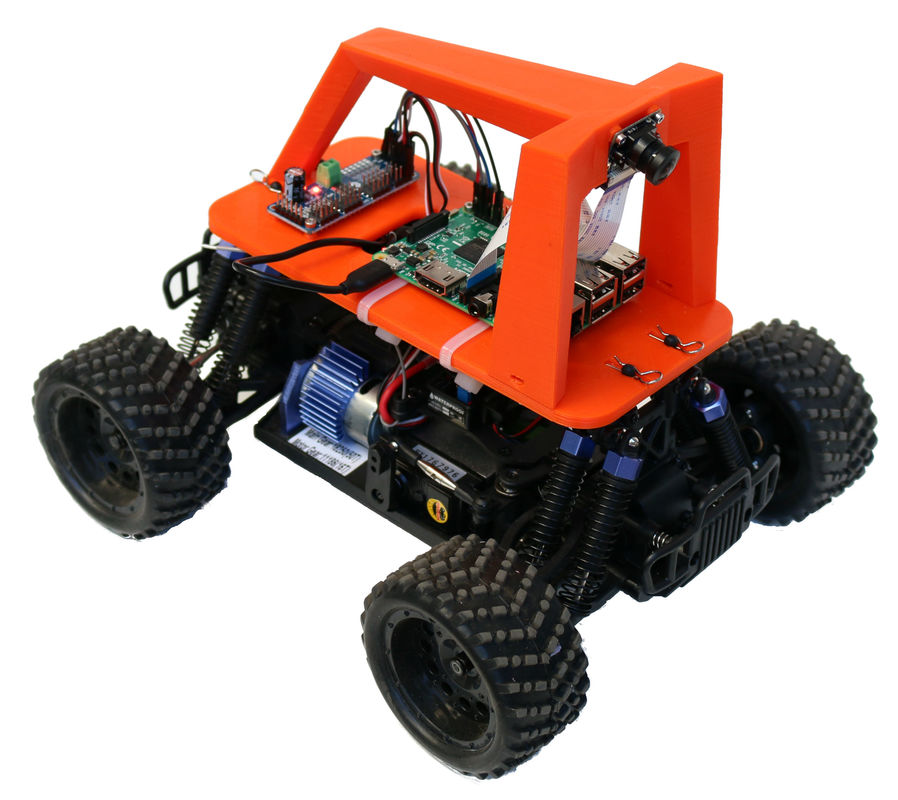
\includegraphics[scale=0.2]{img/donkey.jpg}
\caption{Example of a ``DonkeyCar'', an opensource DIY self driving small car}
\end{figure}

In addition, it's good to know that both thermal motors and cloud computation\footnote{During the race only, training of the model can be done on the cloud} are forbiddens and that the total budget cannot exceed 500\euro{}.

\subsection{Start and Finish}
The car have to be able to start the race by itself after a luminous countdown done by a traffic light of 10x10cm (red, yellow and green). If the car has not start 2 mn after the start, it will be discalified. Each vehicle has the right to a false start, after it will be penalysed. \\

The same way, the vehicule must be able to stop itself maximum 5s after crossing the finish line. This line will be yellow and 15cm long accross the wole width.\\

Any breaches of these rules will result in a penalty:
\begin{itemize}
\item 5s for a false start (after the autorized one)
\item 5s if the car hasn't stop itself in the 5s limits
\end{itemize}

\subsection{Circuit}
The circuit will be made of 2cm wide white marking on top of a 4cm wide black marking on each side of the lane, and will be 45 meters long. Obstacle of 10x10x10cm will be set on the track and could change between each race. The speed is limited to 65km/h.\footnote{Even though it's pretty unlikely that any car can reach this speed in autonomous mode.}\\
So the car must be able to identify those lane and drive without crossing them.\\

\begin{figure}[!h]
\centering
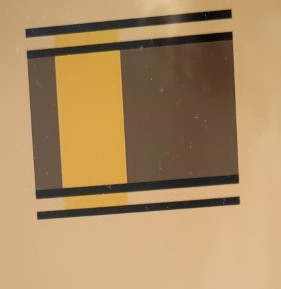
\includegraphics[angle=-90,width=10cm]{img/road.jpeg}
\caption{Representation of the Finish line}
\end{figure}
\clearpage


\section{Project Management}
\subsection{Planning}

The applicative projet only last a semester, but the sigma race is only the $3^{rd}$ of June, so we didn't planned to accomplish all the work only during the \textbf{AP}.\footnote{Short for applicative project} Instead, we decide to focus first on what was the original goal of our AP, driving autonomously in a simulator.\\

As we opted for this AP kind of late\footnote{We first heard of it mid October, we had to think about it, and then we had to do all the proceeding for our inscription.}, we really started working on it arround beginning of November. The first thing to do was to documented ourselves about Machines Learning, Deep Learning, existing software on the domain\dots\\
We gave ourselves a month to gather information about the state of the art in machine learning in autonomous car, but it's such a big domain that we only scratched the surface.


\begin{figure}[!h]
\centering
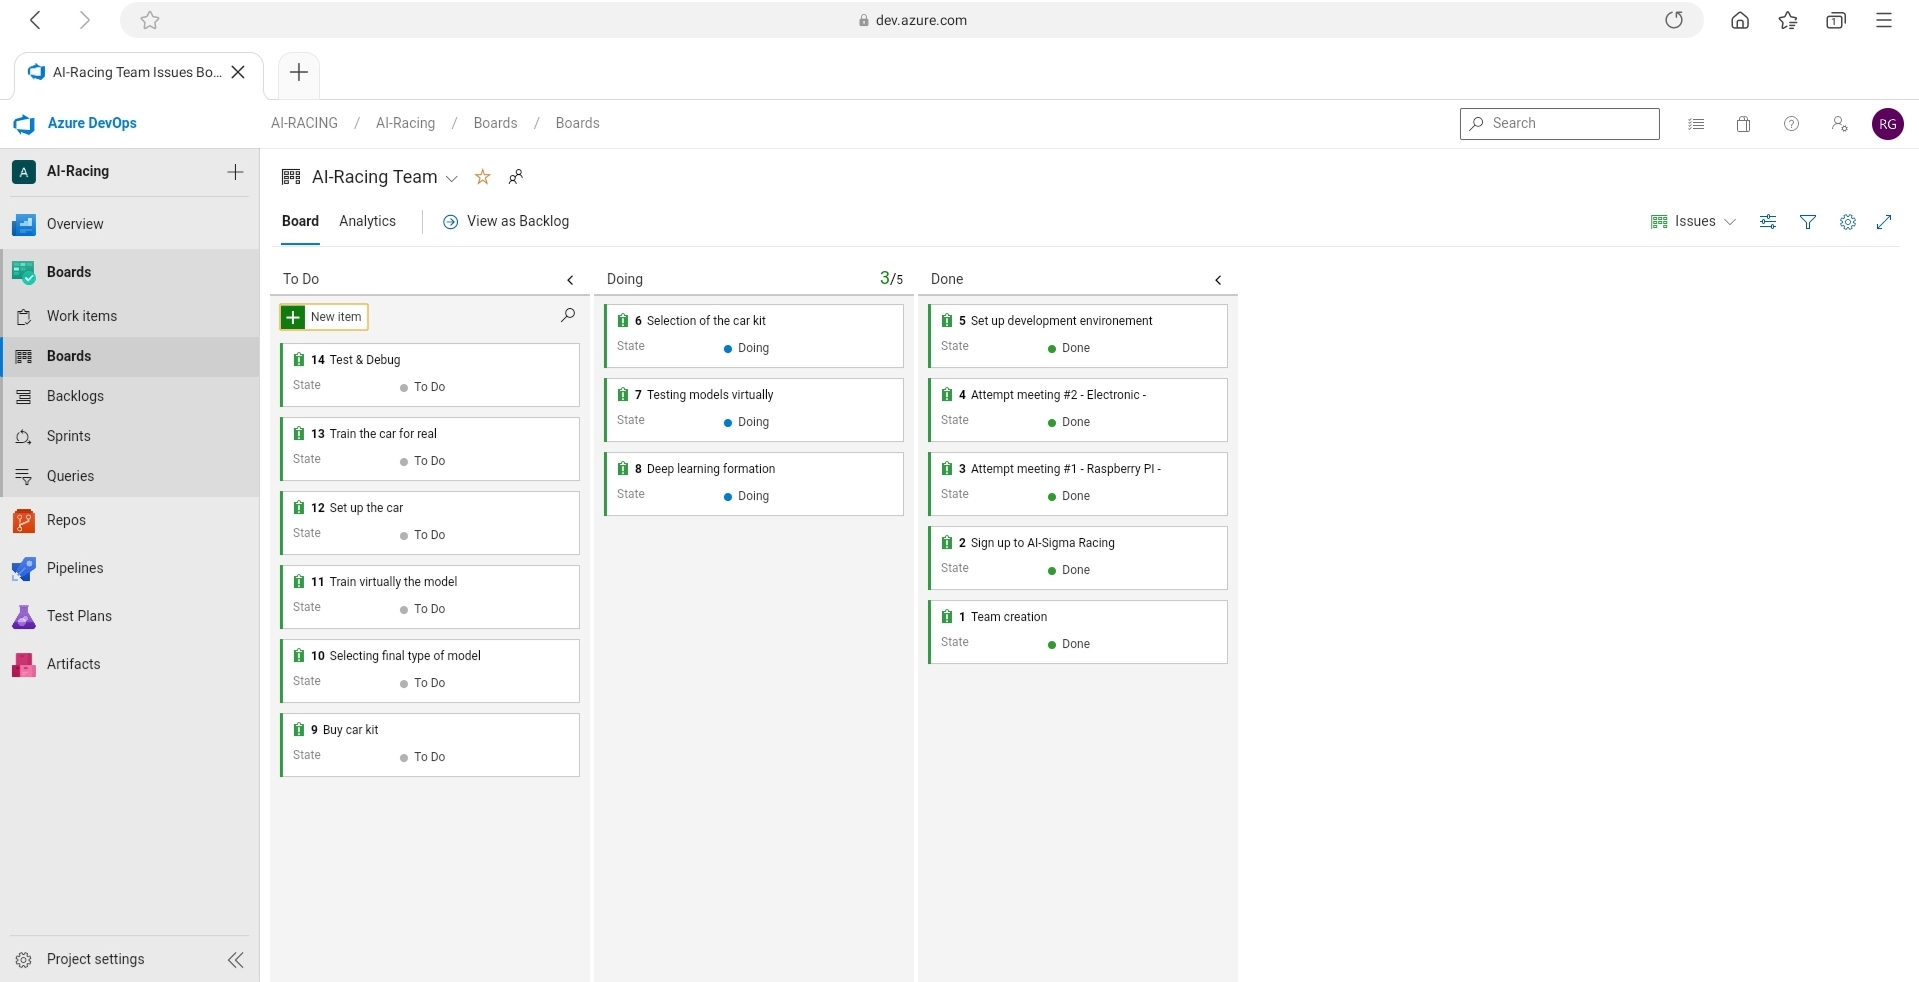
\includegraphics[scale=0.24]{img/devops.jpg}
\caption{We decided to use \textbf{Azure DevOps} to manage our project}
\end{figure}



\subsection{Meetings}
\begin{wrapfigure}{r}{0.4\textwidth}
\centering

\includegraphics[height=5cm]{img/handsonml.jpeg}
\caption{The book Cyprien bought}
\end{wrapfigure}
As we are flatmates, it was pretty easy to do meetings, we used to do a meeting every week or so, in order to share the result of our research. We both start reading book about Machine Learning and Deep Learning in order to understand how this kind of AI are working\cite{2ndEd}.

\clearpage



\begin{figure}[!h]
\centering
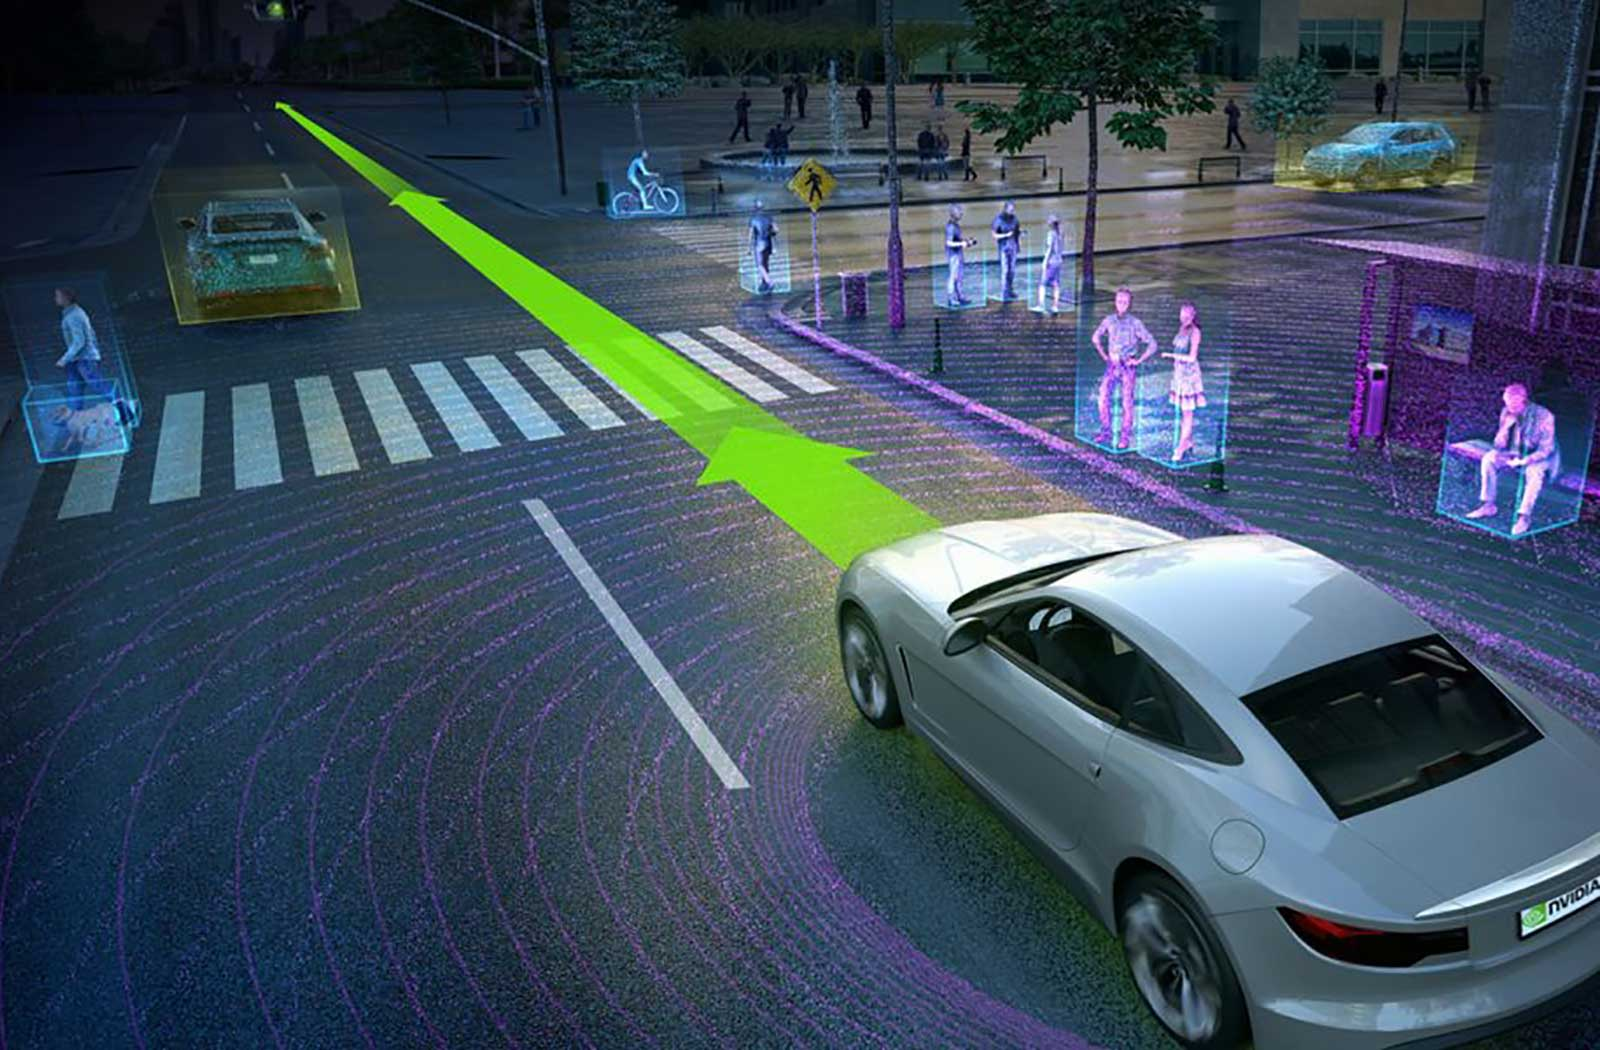
\includegraphics[width=10cm]{img/autonomous_driving.jpeg}
\end{figure}

\subsection{Division of labor}

We divided the work as follow:
\begin{itemize}
\item Cyprien had to setup the simulator
\item Romain had to design a lane detection algorithm 
\item We had to do research on our own to compare deep-learning models to find the best for our situation.
\end{itemize}
\clearpage

\section{Technical overview}

\subsection{DonkeySimulator}

When it comes to simulators, we had 2 options: 
\begin{enumerate}
\item Udacity Simulator
\item DonkeySimulator
\end{enumerate}

\begin{figure}[!h]
\centering
\begin{minipage}[t]{6cm}
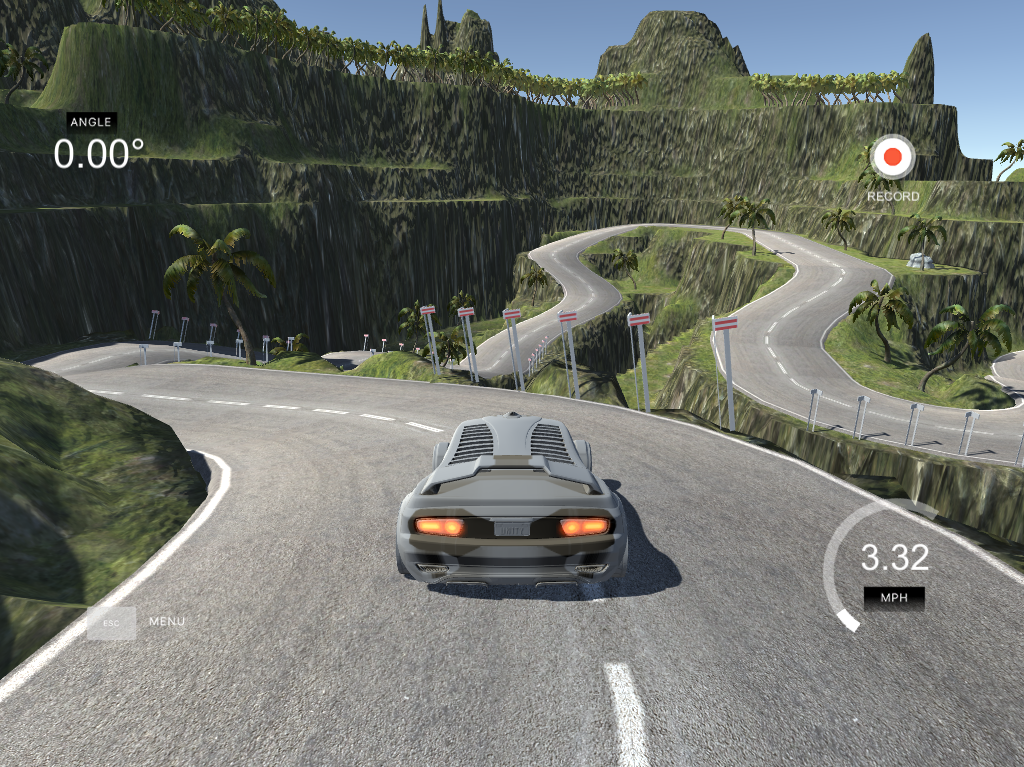
\includegraphics[width=6cm]{img/udacity_sim.png}
\caption{Udacity Simulator}
\end{minipage}
\hspace{1cm}
\begin{minipage}[t]{8cm}
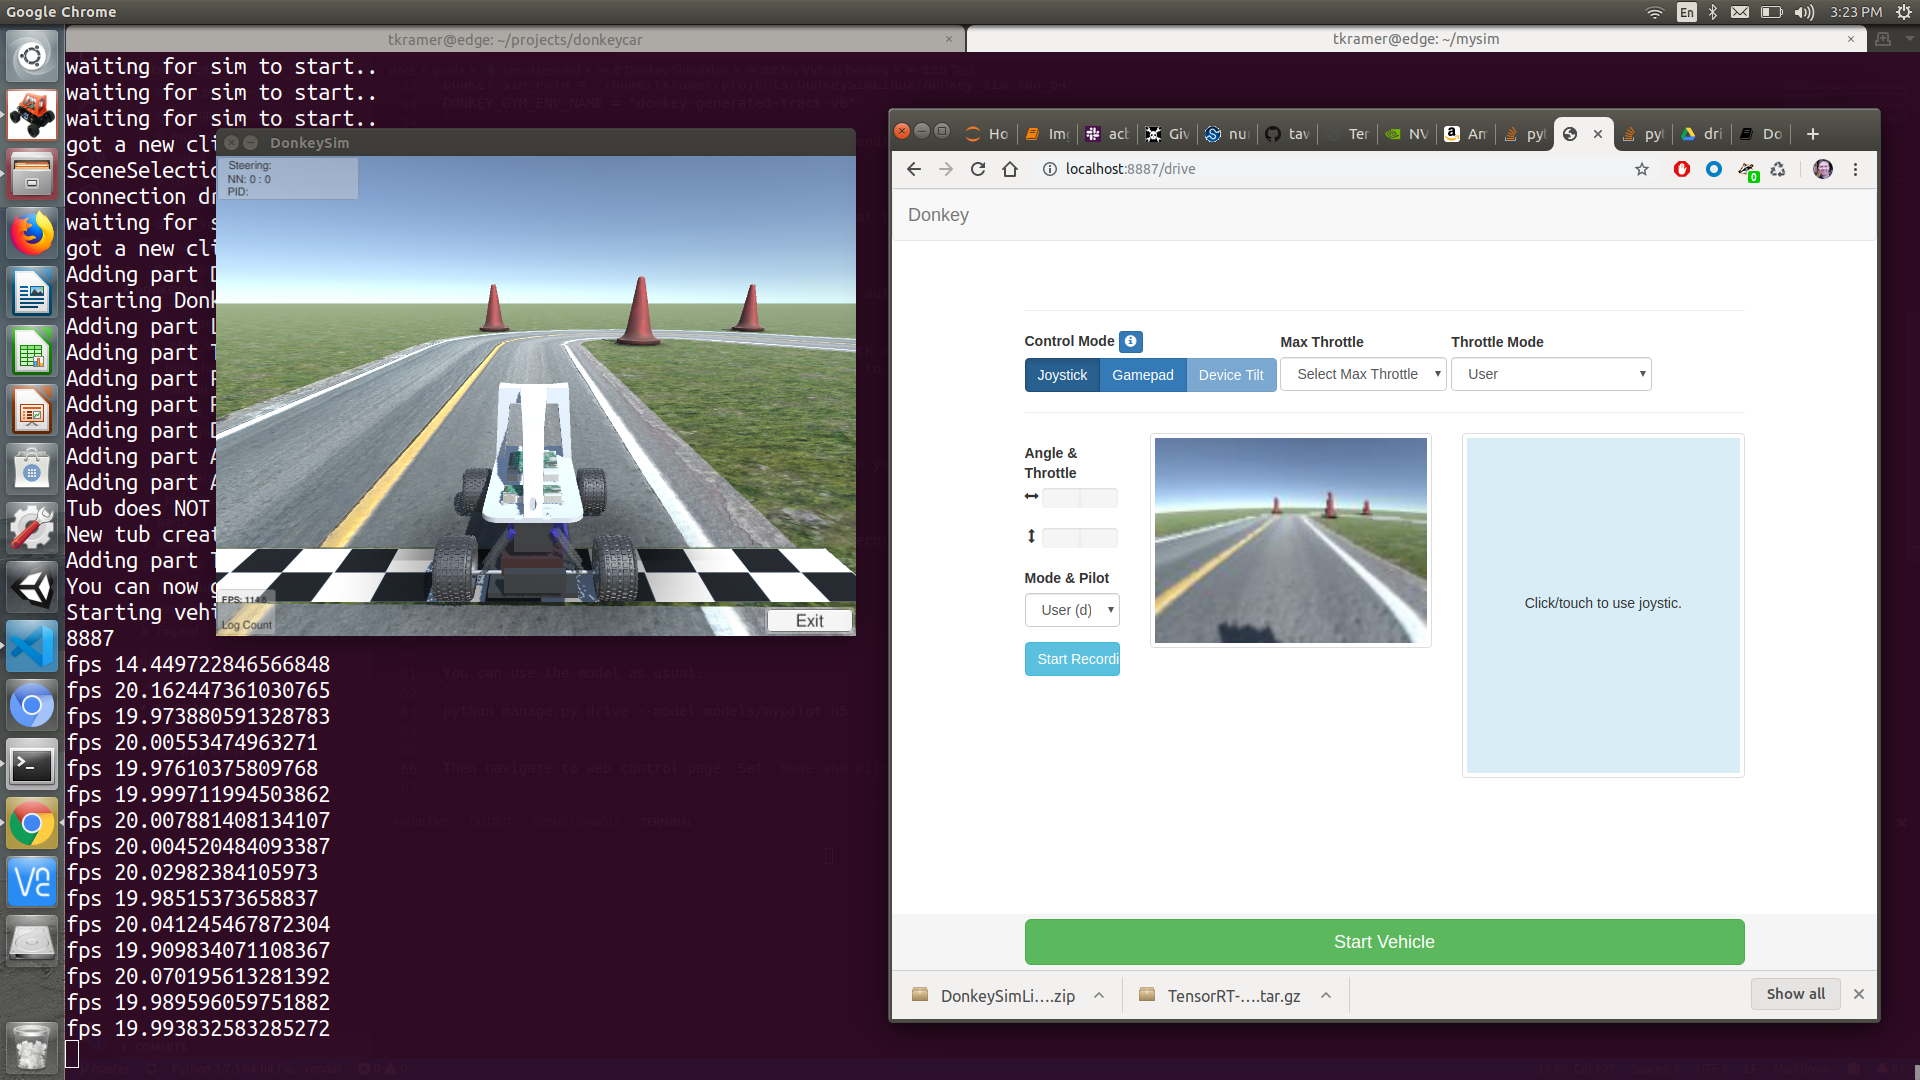
\includegraphics[width=8cm]{img/donkey_sim.png}
\caption{DonkeySimulator}
\end{minipage}
\end{figure}

We decided not to choose the udacity simulator, even though closest to the reality than the DonkeySimulator. ``Why ?'', you may ask. It's because the DonkeySimulator has a built-in track really similar to the one where our car is going to drive the D-day. Moreover, it's easy to implement a second camera to the car, or even simulate the compute power of a \makebox{\textbf{Raspberry pi}}. There's even an OpenAi-Gym environnment !


\begin{figure}[!h]
\centering
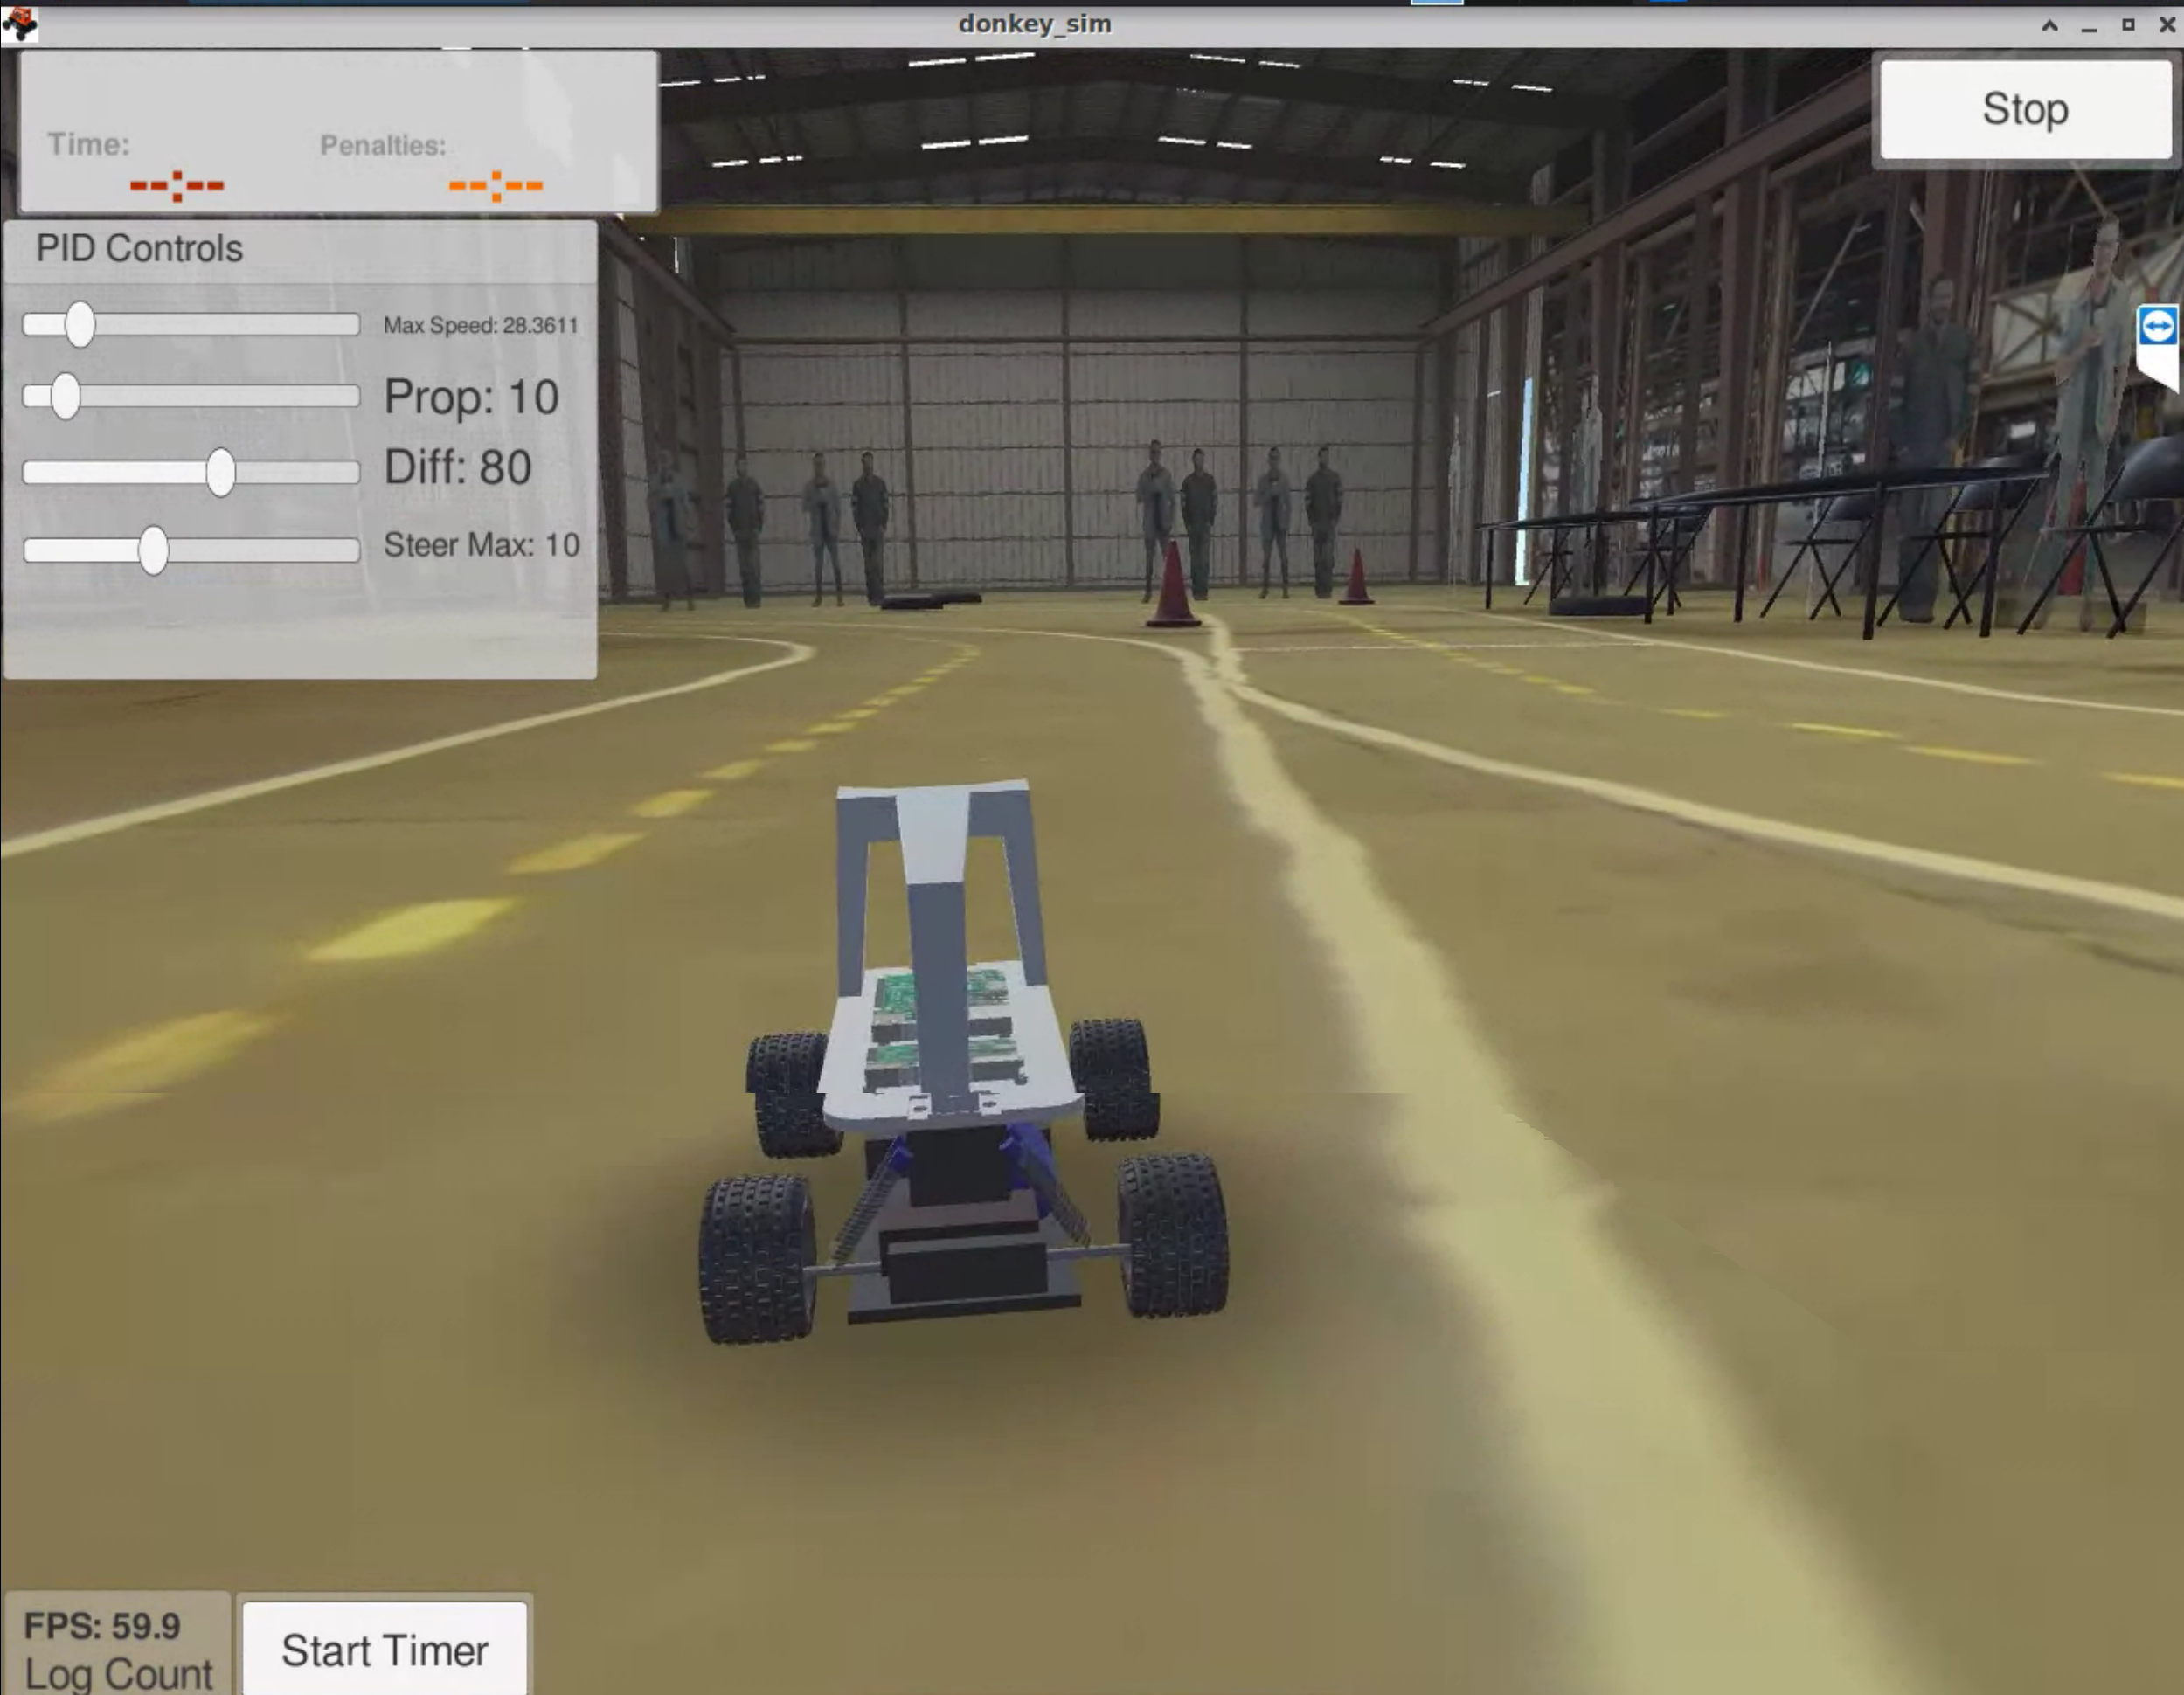
\includegraphics[width=10cm]{img/track.png}
\caption{The track on DonkeySim is really similar to the real one}
\end{figure}
\clearpage

\subsection{Dataset}

We started the project mid-november and we still, at this day, do not have a physic car. In the other hand, we needed to start training models to choose the most efficient. Our only option was to find online dataset to start training a model, and then, when we'll receive the car, we'll just have to transfer it in the car.\\





\subsection{Our model choice}

First we need to plant the basics. What our AI model needs to make predictions on ? Our model will make live predictions on the steering and the throttle of our car using images given by the camera on the car.\\

What is the best algorithm ? Which one is the most relaible, efficient ?\\

We have several options and this part, we will present the pros and the cons of the algorithm selection that we have made.\\

We will be using the Keras (open-source sofware library with a python interface) high level API in combination with a Tensorflow backend.\\ 

\subsubsection*{Keras Categotical}

\begin{table}[!h]
\begin{center}
\begin{tabular}{|p{6cm}|p{6cm}|}
\hline
\textbf{Pros} & \textbf{Cons}\\
\hline
It has some benefits of showing the confidense as a distribution via the makemovie command & Suffers from some arbitrary limitations of the chosen limits for number of categories, and thottle upper limit \\
\hline
It has been very robust & \\
\hline
In some cases this model has learned thottle control better than other models & \\
\hline
Performs well in a limited compute environment like the Pi3 & \\
\hline
\end{tabular}
\end{center}
\caption{Keras Categorical Pros/Cons}
\end{table}



\subsubsection*{Keras Linear}

\begin{table}[!h]
\begin{center}
\begin{tabular}{|p{6cm}|p{6cm}|}
\hline
\textbf{Pros} & \textbf{Cons}\\
\hline
Steers smoothly & May sometimes fail to learn throttle well \\
\hline
It has been very robust & \\
\hline
No arbitrary limits to steering or throttle  & \\
\hline
Performs well in a limited compute environment like the Pi3 & \\
\hline
\end{tabular}
\end{center}
\caption{Keras Linear Pros/Cons}
\end{table}

\subsubsection*{Keras IMU}

\begin{table}[H]
\begin{center}
\begin{tabular}{|p{6cm}|p{6cm}|}
\hline
\textbf{Pros} & \textbf{Cons}\\
\hline
Steers very smoothly  & Driving quality will suffer if noisy imu is used \\
\hline
Performs well in a limited compute environment like the Pi3  & \\
\hline
No arbitrary limits to steering or throttle  & \\
\hline
Gives additional state to the model, which might help it come to a stop at a stop sign & \\
\hline
\end{tabular}
\end{center}
\caption{Keras IMU Pros/Cons}
\end{table}


\subsubsection*{Keras Latent}

\begin{table}[H]
\begin{center}
\begin{tabular}{|p{6cm}|p{6cm}|}
\hline
\textbf{Pros} & \textbf{Cons}\\
\hline
Steers smoothly  & Needs more testing to prove theory  \\
\hline
Performs well in a limited compute environment like the Pi3  & \\
\hline
No arbitrary limits to steering or throttle.  & \\
\hline
Image output a measure of what the model has deemed important in the scene & \\
\hline
\end{tabular}
\end{center}
\caption{Keras Latent Pros/Cons}
\end{table}

\subsubsection*{Keras RNN}

\begin{table}[H]
\begin{center}
\begin{tabular}{|p{6cm}|p{6cm}|}
\hline
\textbf{Pros} & \textbf{Cons}\\
\hline
Steers very smoothly  & Performs worse in a limited compute environment like the Pi3\\
\hline
Can train to a lower loss   & Takes longer to train \\
\hline
\end{tabular}
\end{center}
\caption{Keras RNN Pros/Cons}
\end{table}


\subsubsection*{Keras Behaviour}

\begin{table}[H]
\begin{center}
\begin{tabular}{|p{6cm}|p{6cm}|}
\hline
\textbf{Pros} & \textbf{Cons}\\
\hline
Can create a model which can perform multiple tasks & Takes more effort to train \\
\hline
\end{tabular}
\end{center}
\caption{Keras Behaviour Pros/Cons}
\end{table}

\subsubsection*{Keras Localizer}

\begin{table}[H]
\begin{center}
\begin{tabular}{|p{6cm}|p{6cm}|}
\hline
\textbf{Pros} & \textbf{Cons}\\
\hline
Steers smoothly  & May sometimes fail to learn throttle well  \\
\hline
Performs well in a limited compute environment like the Pi3  & \\
\hline
No arbitrary limits to steering or throttle.  & \\
\hline
Location to supply some higher level logic & \\
\hline
\end{tabular}
\end{center}
\caption{Keras Localizer Pros/Cons}
\end{table}


\subsection{Lane Detection algorithm}

The first to do was to create a simple lane detection algorithm, by assuming that all line will be straight. We used \textbf{OpenCV}, an open-source computer vision library, usable both in Python and C++. This tool include image processing, camera calibration, object detection\dots \\

\begin{figure}[!h]
\centering

\includegraphics[scale=0.25]{img/opencv.png}
\caption{OpenCV is an Open-source Computer Vision Library}
\end{figure}

The usual methodology in this case is as follow:\footnote{Cf. appendix \ref{laneDetect} for the complete code and appendix \ref{imagelaneDetect} for the pictures}
\begin{enumerate}
\item Put image in gray in order to emphasize the white lines
\item Blur the immage using a \textbf{Gaussian Filter}\footnote{By averaging the values of nearby pixels, the Gaussian Filter reduce the noise in the image}
\item Use the \textbf{Canny} algorithm to find edges on the image
\item Cropp the image only where the lines should be
\item Using the \textbf{Hough} algorithm to find lines in the resulted image
\item Select the average left line and right line from the array of lines
\item Finaly display the line on top of the image (or frame in case of a video)
\end{enumerate}



\clearpage
\subsection{OpenAI Gym}

\begin{figure}[!h]
    \centering
    \def\svgwidth{0.7\columnwidth}
    \input{openai.pdf_tex}
\end{figure}

OpenAI, one of the most famous company in the Deep Learning domain, has developped an open-source framework to help the implementation of a certain type of deep learning algorithm. This kind of algorithm is particularly efficient when it comes to\dots~playing games !\\

In fact, OpenAi-Gym is best suited for \textbf{Reinforcement Learning}, a genre of neural network were the agent is rewarded when taking good actions and penalized when doing bad things. These neural network are complicated to implement in the real world, imagine a car having to crash thousands of time before learning to turn left ! But that doesn't mean they are bad ! In fact, it's kind of the opposite: remember \textbf{AlphaGo Zero} ? It's the first algorithm to defeat the world champion of Go\footnote{Go is a game with more than $10^{17}$ possible board configuration\cite{AlphaGo}} in a 1vs1 match, and it was using reinforcment learning !\\

\subsubsection*{Reinforcement Learning}
\begin{figure}[!h]
\centering
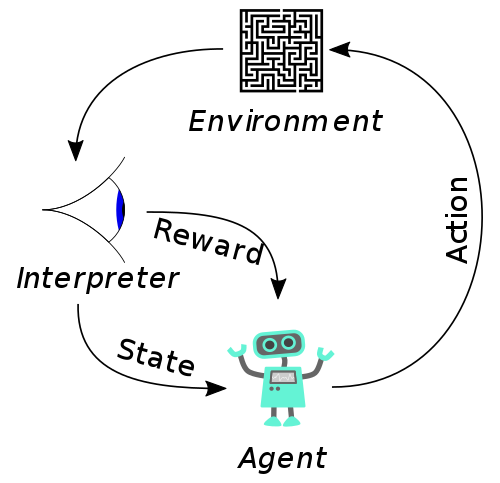
\includegraphics[width=10cm]{img/Reinforcement_learning_diagram.png}
\caption{Schematic of the reinforcement learning algorithm}
\end{figure}
\clearpage

In order to train a Reinforcement Neural Network, we have to provide it 2 differents things at each step:
\begin{itemize}
\item A state
\item A reward
\end{itemize}
And the neural network will output an action which is going to have an impact on the environment. Then the loop repeat itself.\\

In \textbf{Python}, OpenAi Gym is implemented as follow:

\subsubsection*{OpenAi Gym in Python \cite{OpenAI}}
\texttt{Steps} stipulate how long the networks is going to run (it has to be an Integer). At each step, \texttt{Observation}, \texttt{Reward}, \texttt{Done} and \texttt{Info} are outputed.\\

\texttt{Observation} represent all the data fed to the agent at a given step, it can be pixel data such as in a picture, speed, memory.\footnote{One of the goal of OpenAi Gym was to make an AI able to beat most of the NES game with only the raw memory as observation} The observation differ depending on the task, so it's taking the form of an \texttt{object}.\\

\texttt{Reward} is a \texttt{float}, positive or not, given to the agent after he took an action. The goal of the agent is to maximise the total reward.\\

\texttt{Done} is a \texttt{boolean}. When set to \texttt{True}, it indicate that the episode has terminated (either the task has failed, or the task was successfuly handled).\\

\texttt{Info} is a \texttt{dictionnary} containing information for the developper (often used for debuging). The agent is not allowed to access these informations.\\

\texttt{Space} is either a \texttt{set} or a \texttt{box}\footnote{Depending if the action space is continous or discrete} containing all the possible \texttt{Actions} that the agent can take.\\

\begin{figure}[!h]
\centering
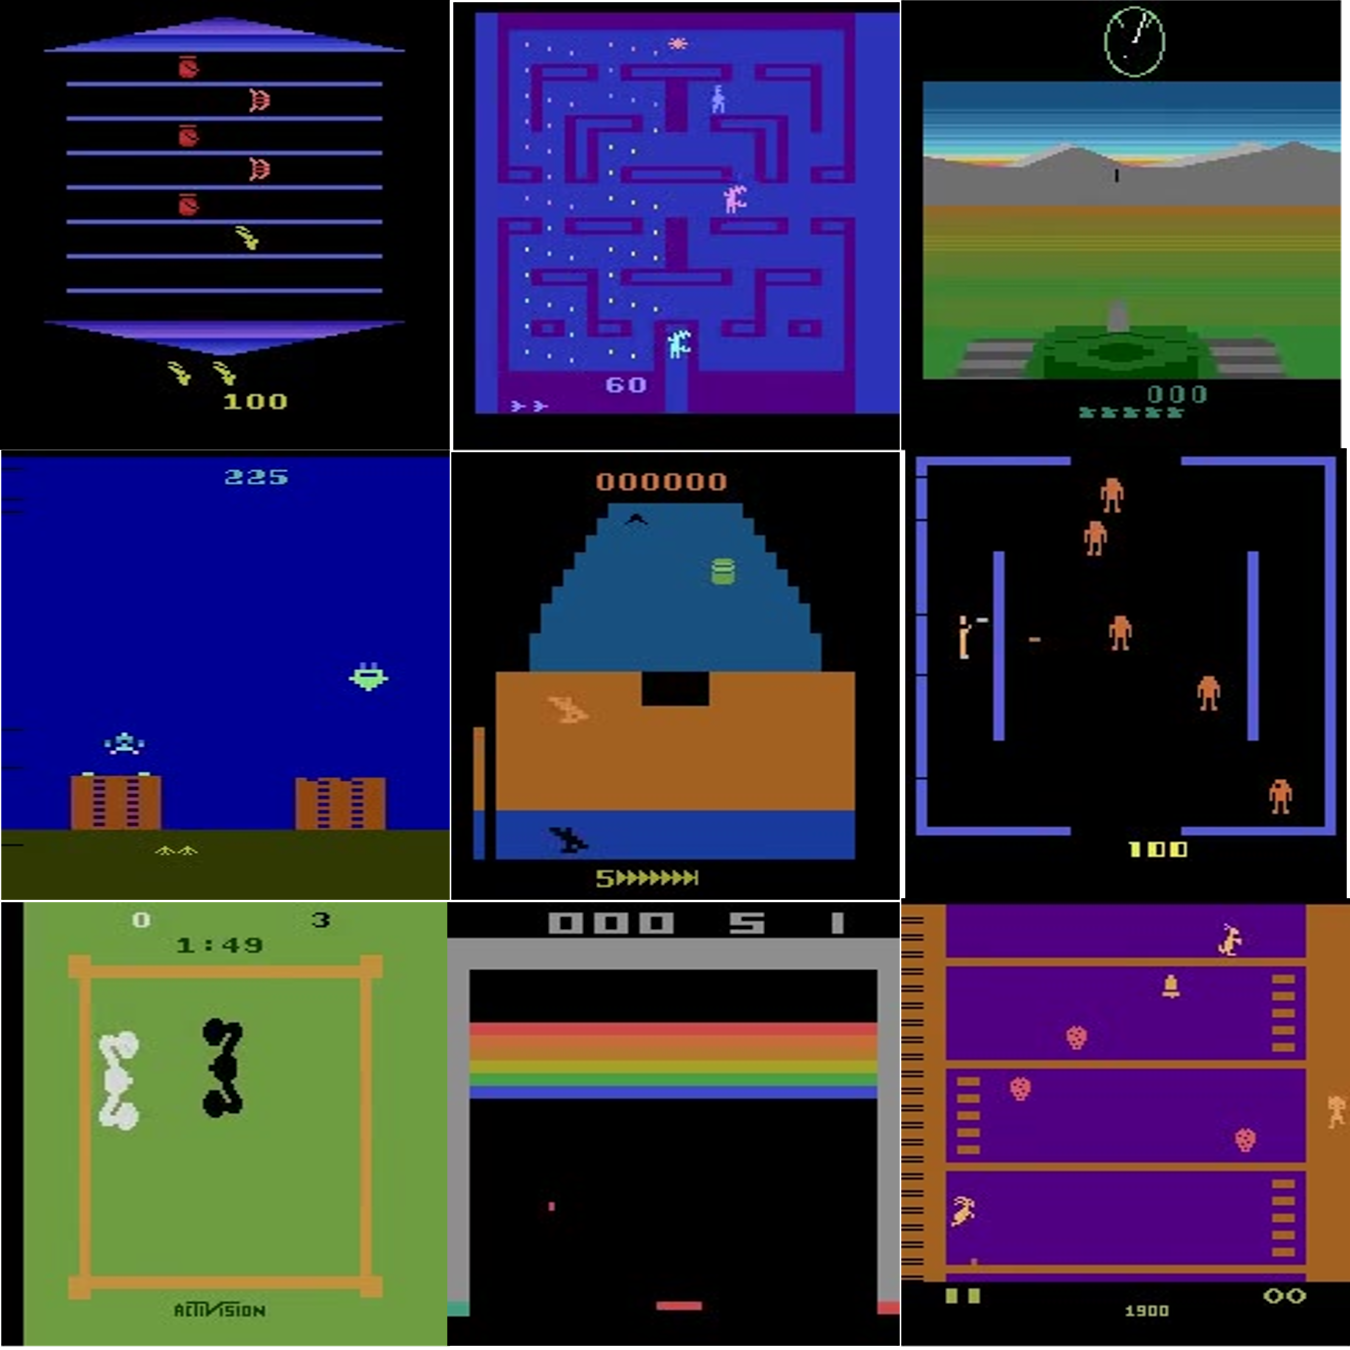
\includegraphics[scale=0.15]{img/openai_gym_environment.png}
\caption{Different kind of Atari Games environment available in OpenAi-Gym}
\end{figure}
\clearpage

\hfill \\
This framework makes it really easy to implement RNN in environment well formated. Fortunatly, the community have already build a OpenAI-Gym environment for the DonkeySimulator: Gym-Donkeycar


\subsubsection*{Gym DonkeyCar}

Thanks to Tawn KRAMER\cite{GymDonkey}, we have a pre-made environment following the OpenAI-Gym methodology. It basically runs a TCP connection with the simulator and transform the data received into Python formated data. This way, we don't have to create the TCP client by ourself\footnote{Although we tried doing it cf. appendix \ref{TCPClient}}

 The same component are implemented as follow:\\

\texttt{Observation} is a \texttt{np.array} with a shape of (120, 160, 3).\footnote{Basicaly it's the RGB representation of a 120x160px image}\\

\texttt{Done} is a \texttt{boolean} set to \texttt{True} when the car hit an obstacle (\texttt{hit != "none"}) or when it's too far from the center of the lane.\\

\texttt{Reward} is an \texttt{array} containing \texttt{Done}, the \textbf{speed}\footnote{Between max=1 and min=-2} of the vehicule and the \textbf{Cross Track error} (cte)\footnote{How far the car is from the center of the lane}\\

\texttt{Info} is an \texttt{array} containing the \textbf{cte}, the \textbf{position} (x,y,z), the \textbf{speed} (positive forward, negative backward) and if the car has it an obstacle: \textbf{hit}  (equal to "none" if all good)\cite{DonkeySim}

With all these information, we can feed the network with the \texttt{Observation} and make it output a steering angle and a throtle value.\\

It's quite funny to watch the IA train, because it's basically running all over the place at first, but then it start going further and further on the track. Sometimes you can have a big gain from a step to an other, or the AI can even regress ! But in the end, after a few hours of training, the AI is finaly able to drive through the whole track !

\begin{figure}[H]
\centering
\begin{minipage}{6cm}
\centering
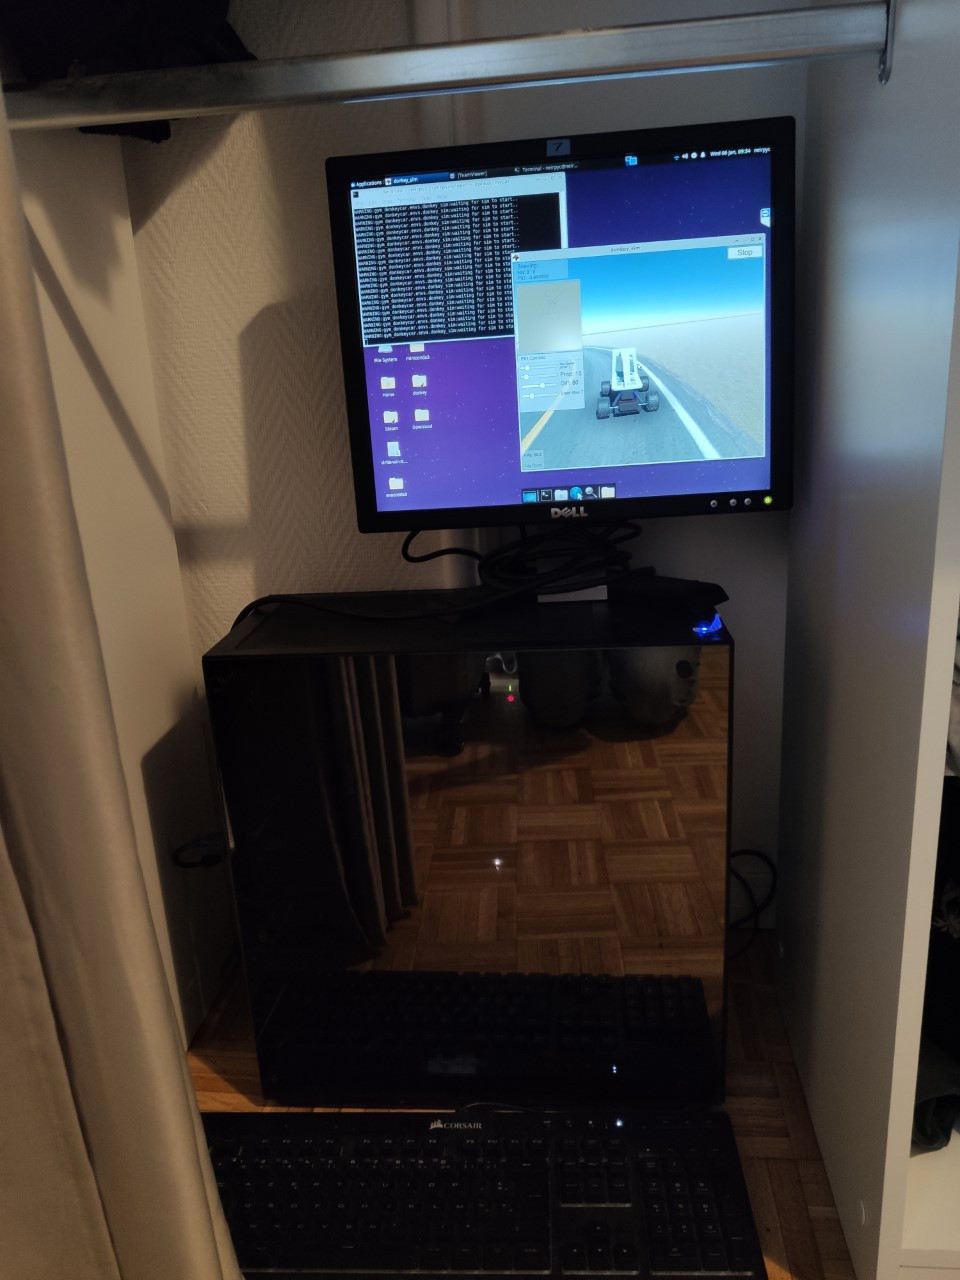
\includegraphics[scale=0.13]{img/linux.jpeg}
\caption{The Linux server we used for our training : \makebox{Xeon X5650 (6 cores 12 threads)}  8Go DDR3 - Nvidia GTX 970 4Go}
\end{minipage}
\hspace{2cm}
\begin{minipage}{6cm}
\centering
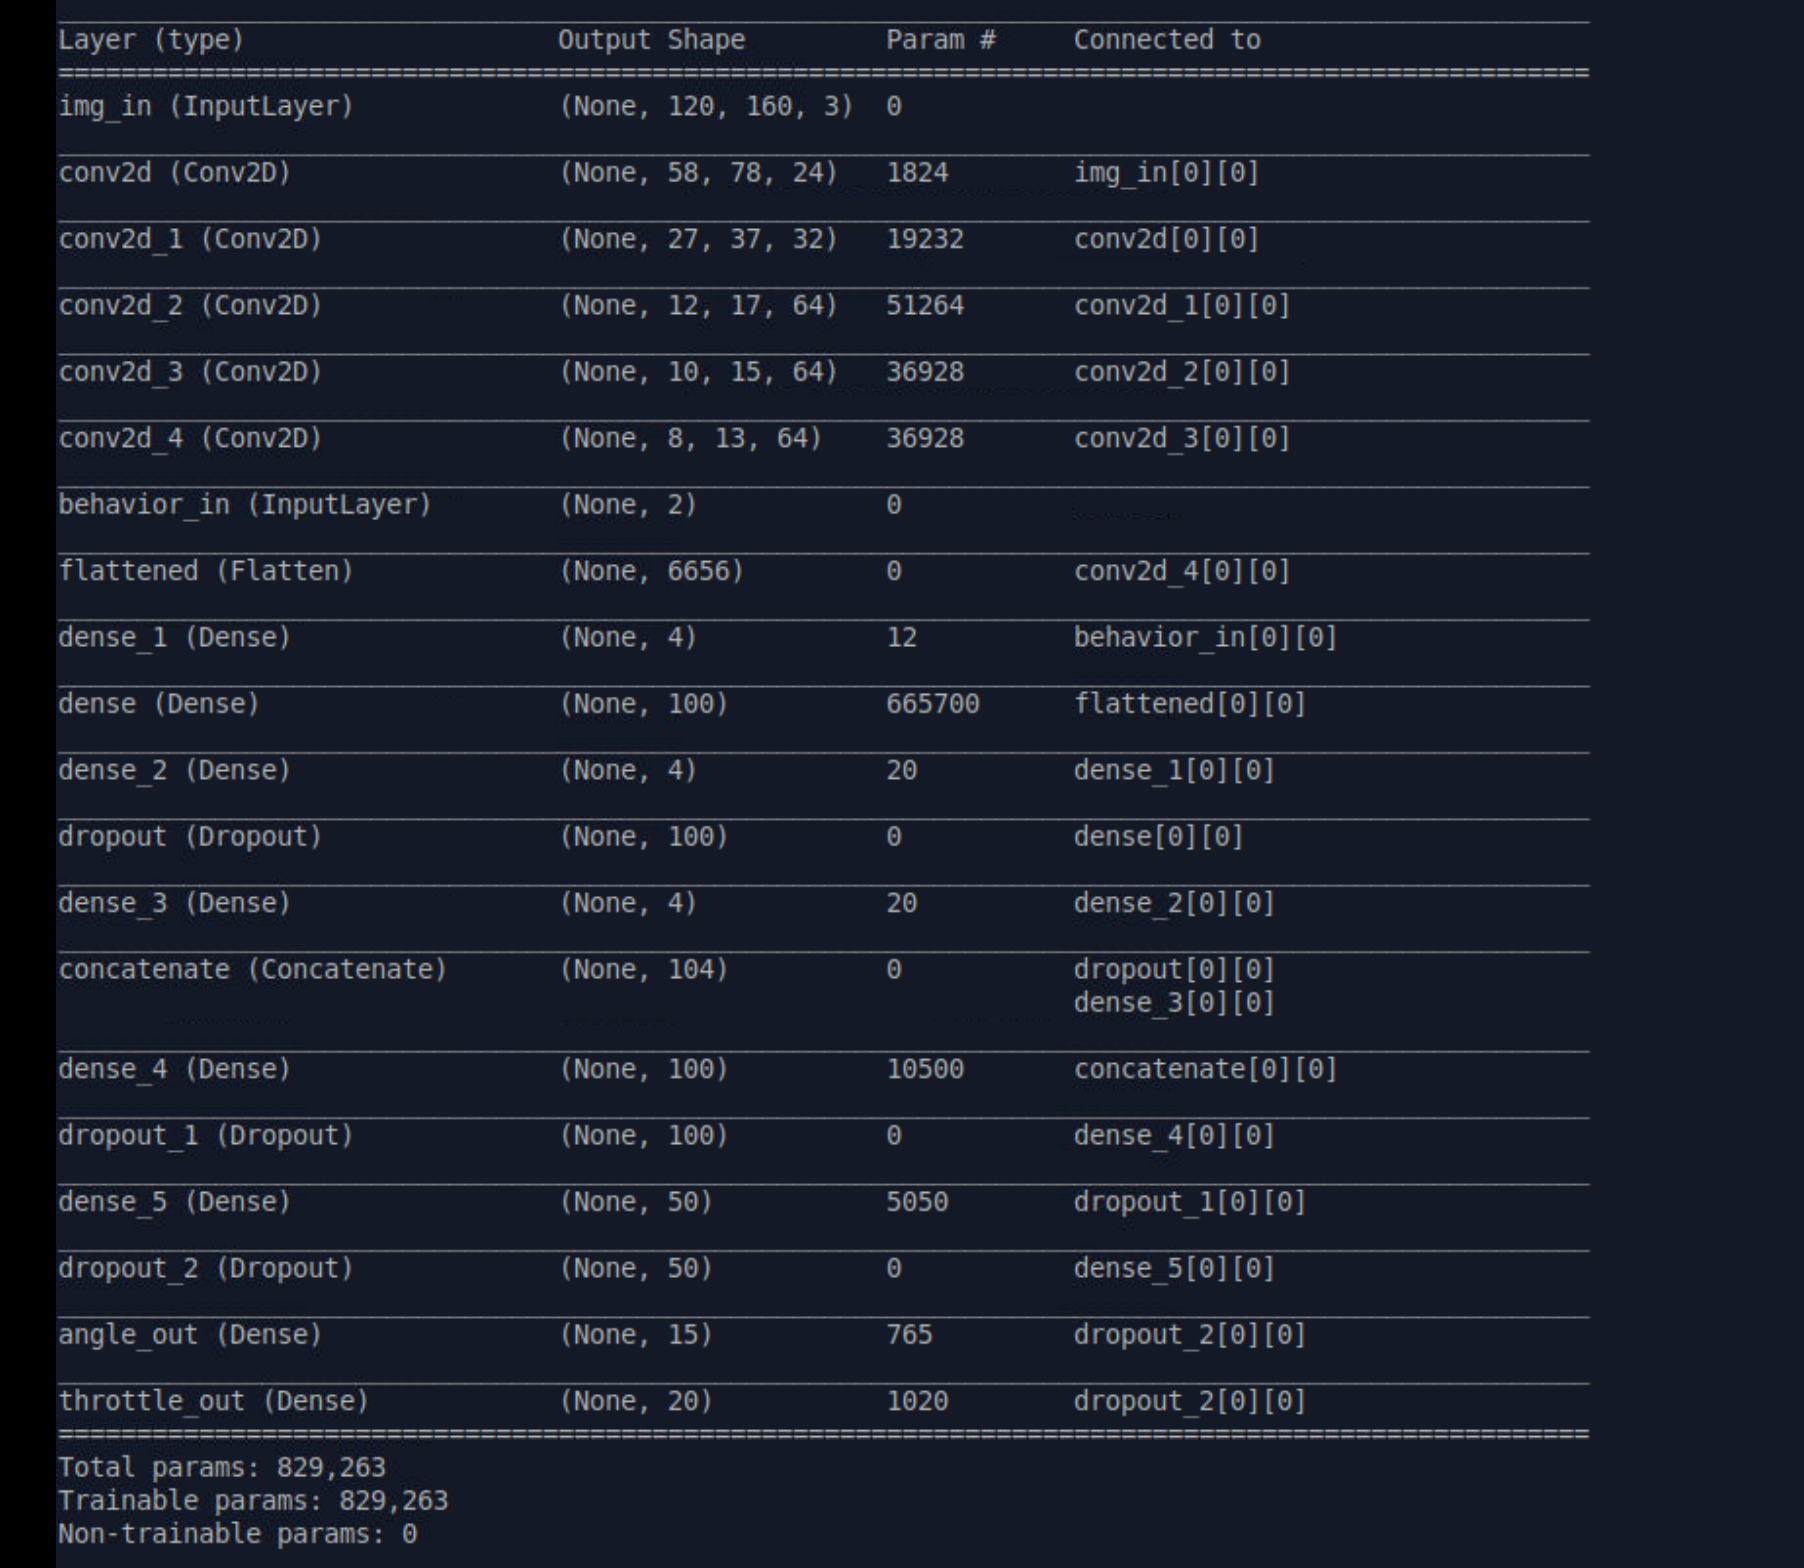
\includegraphics[scale=0.13]{img/keras.png}
\caption{example model run}
\end{minipage}
\end{figure}

\clearpage
\subsection{Benchmarks}

Using the DonkeySimulator, we ran 4 differents algorithms (unfortunatly we were not able to compute neither the imu nor the behaviour model), all in the same conditions, in order to compare their performances :\\
We used 9143 training images that we split in 7314 training images and 1829 validation images. 57 steps have been run each epoch.


\begin{figure}[!h]
\begin{minipage}{8cm}
\centering
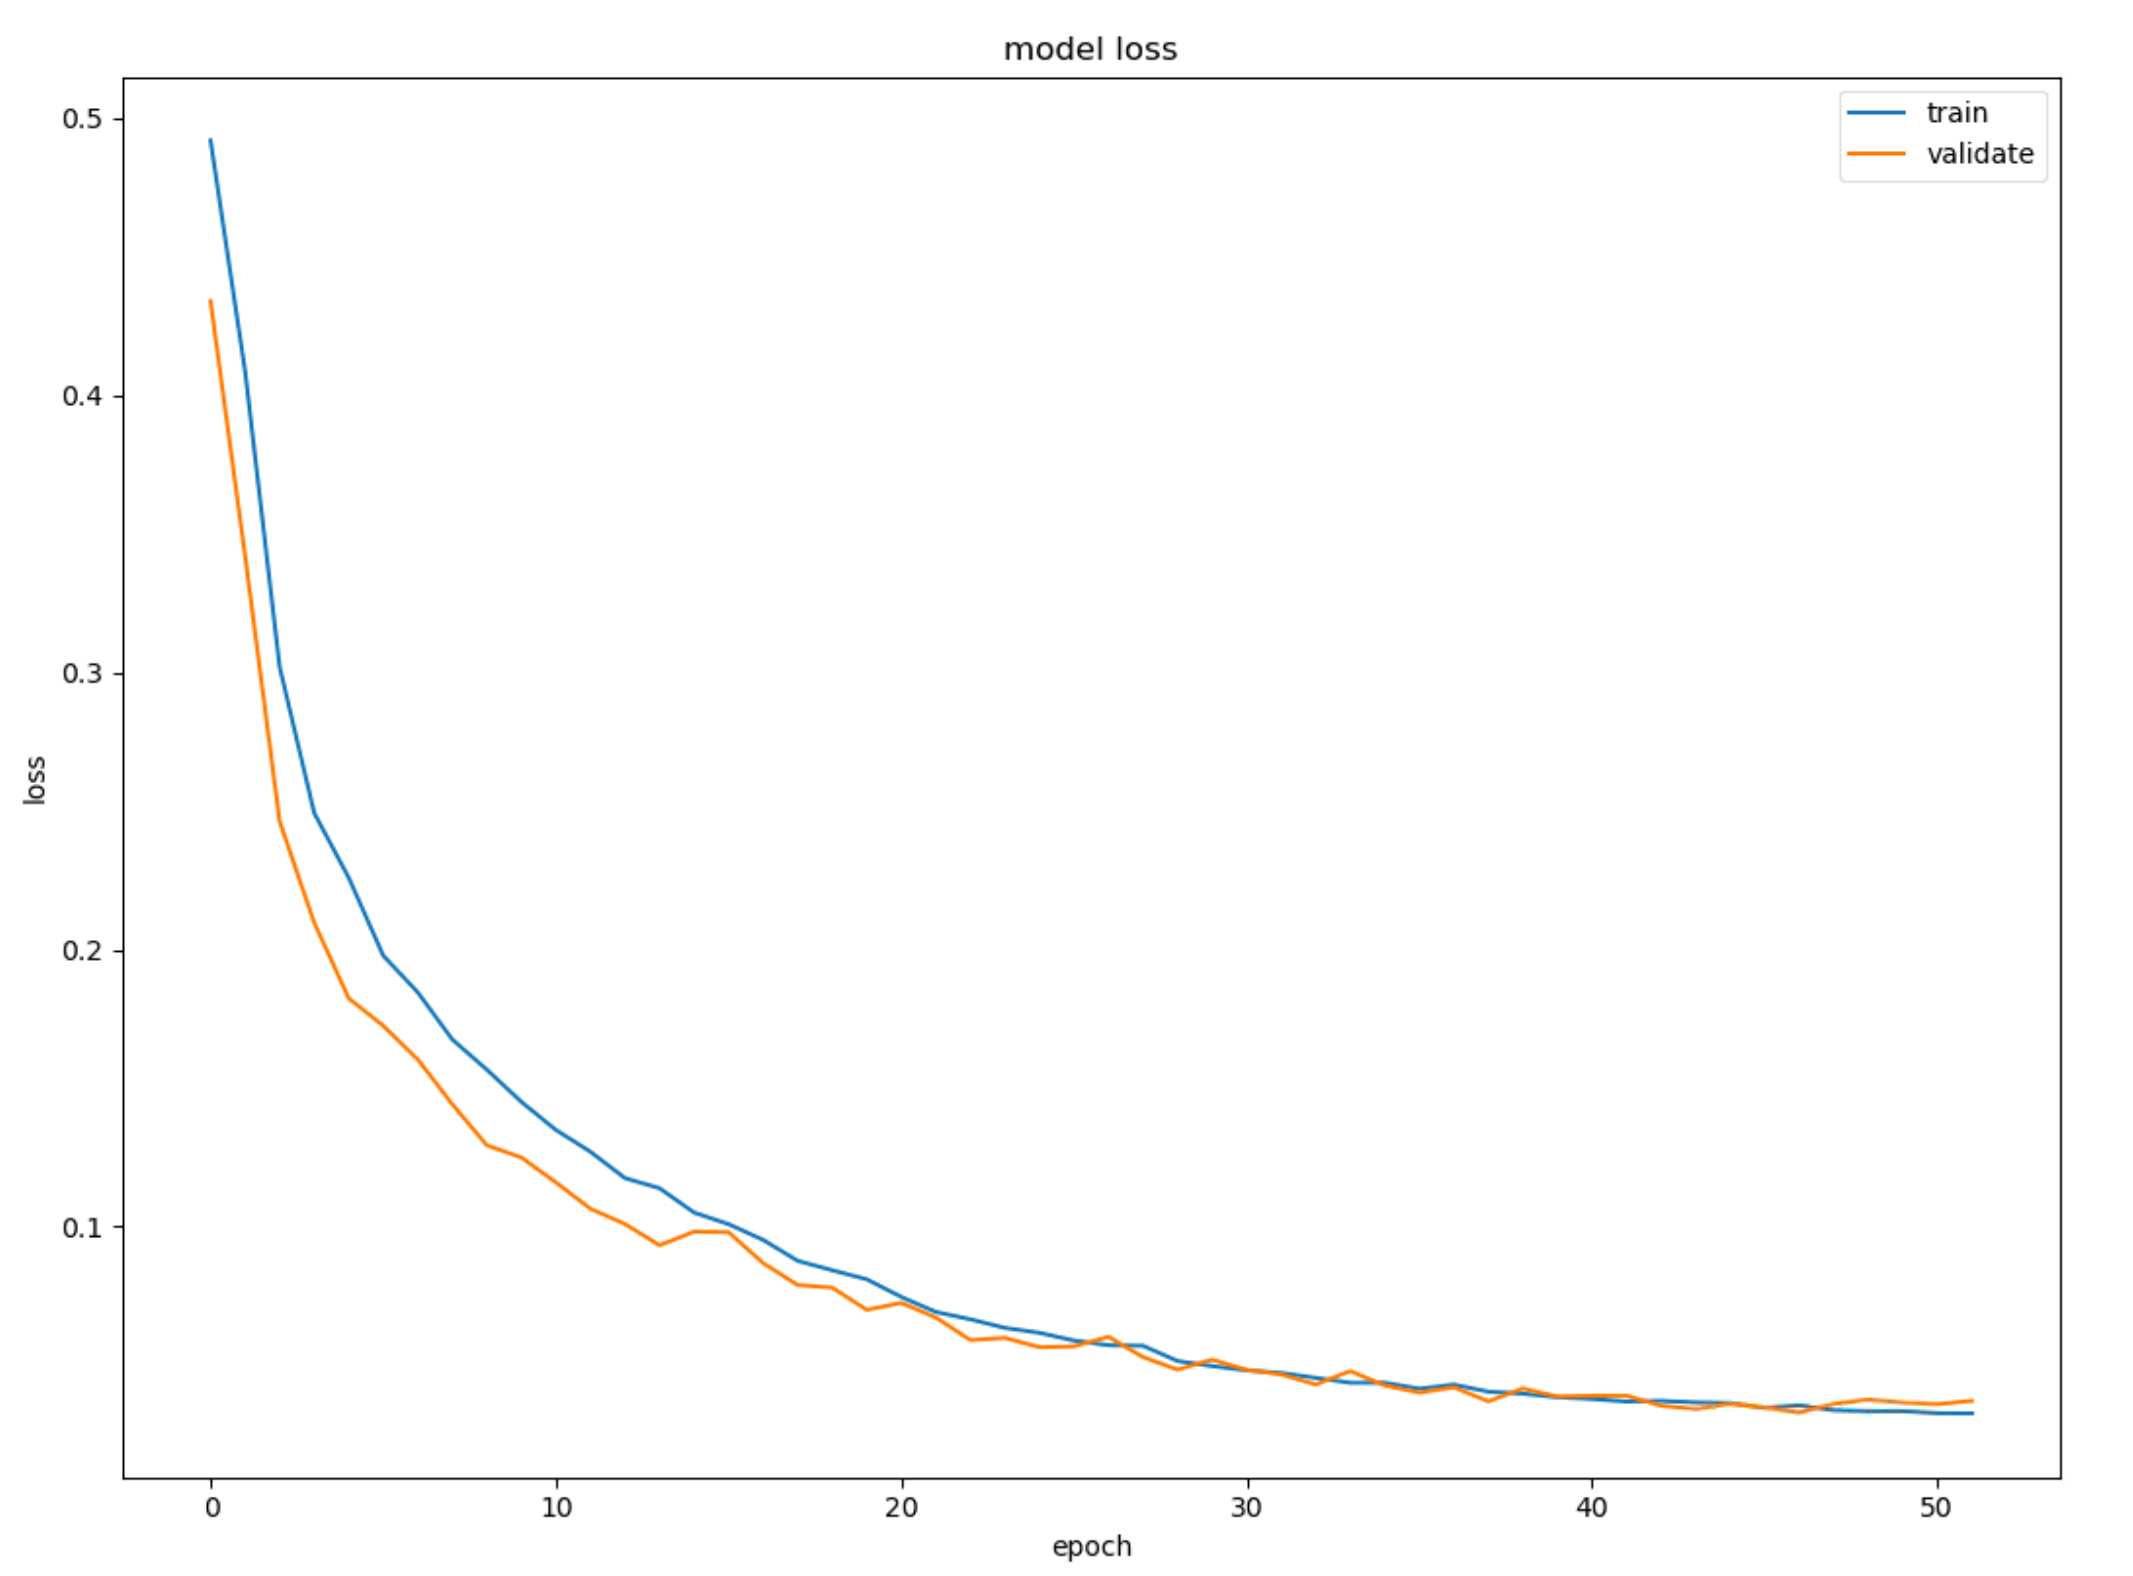
\includegraphics[width=8cm]{img/model_bench/linear.png}
\caption{Linear model loss}
\label{Linear model loss}
\end{minipage}
\hspace*{1cm}
\begin{minipage}{8cm}
\centering
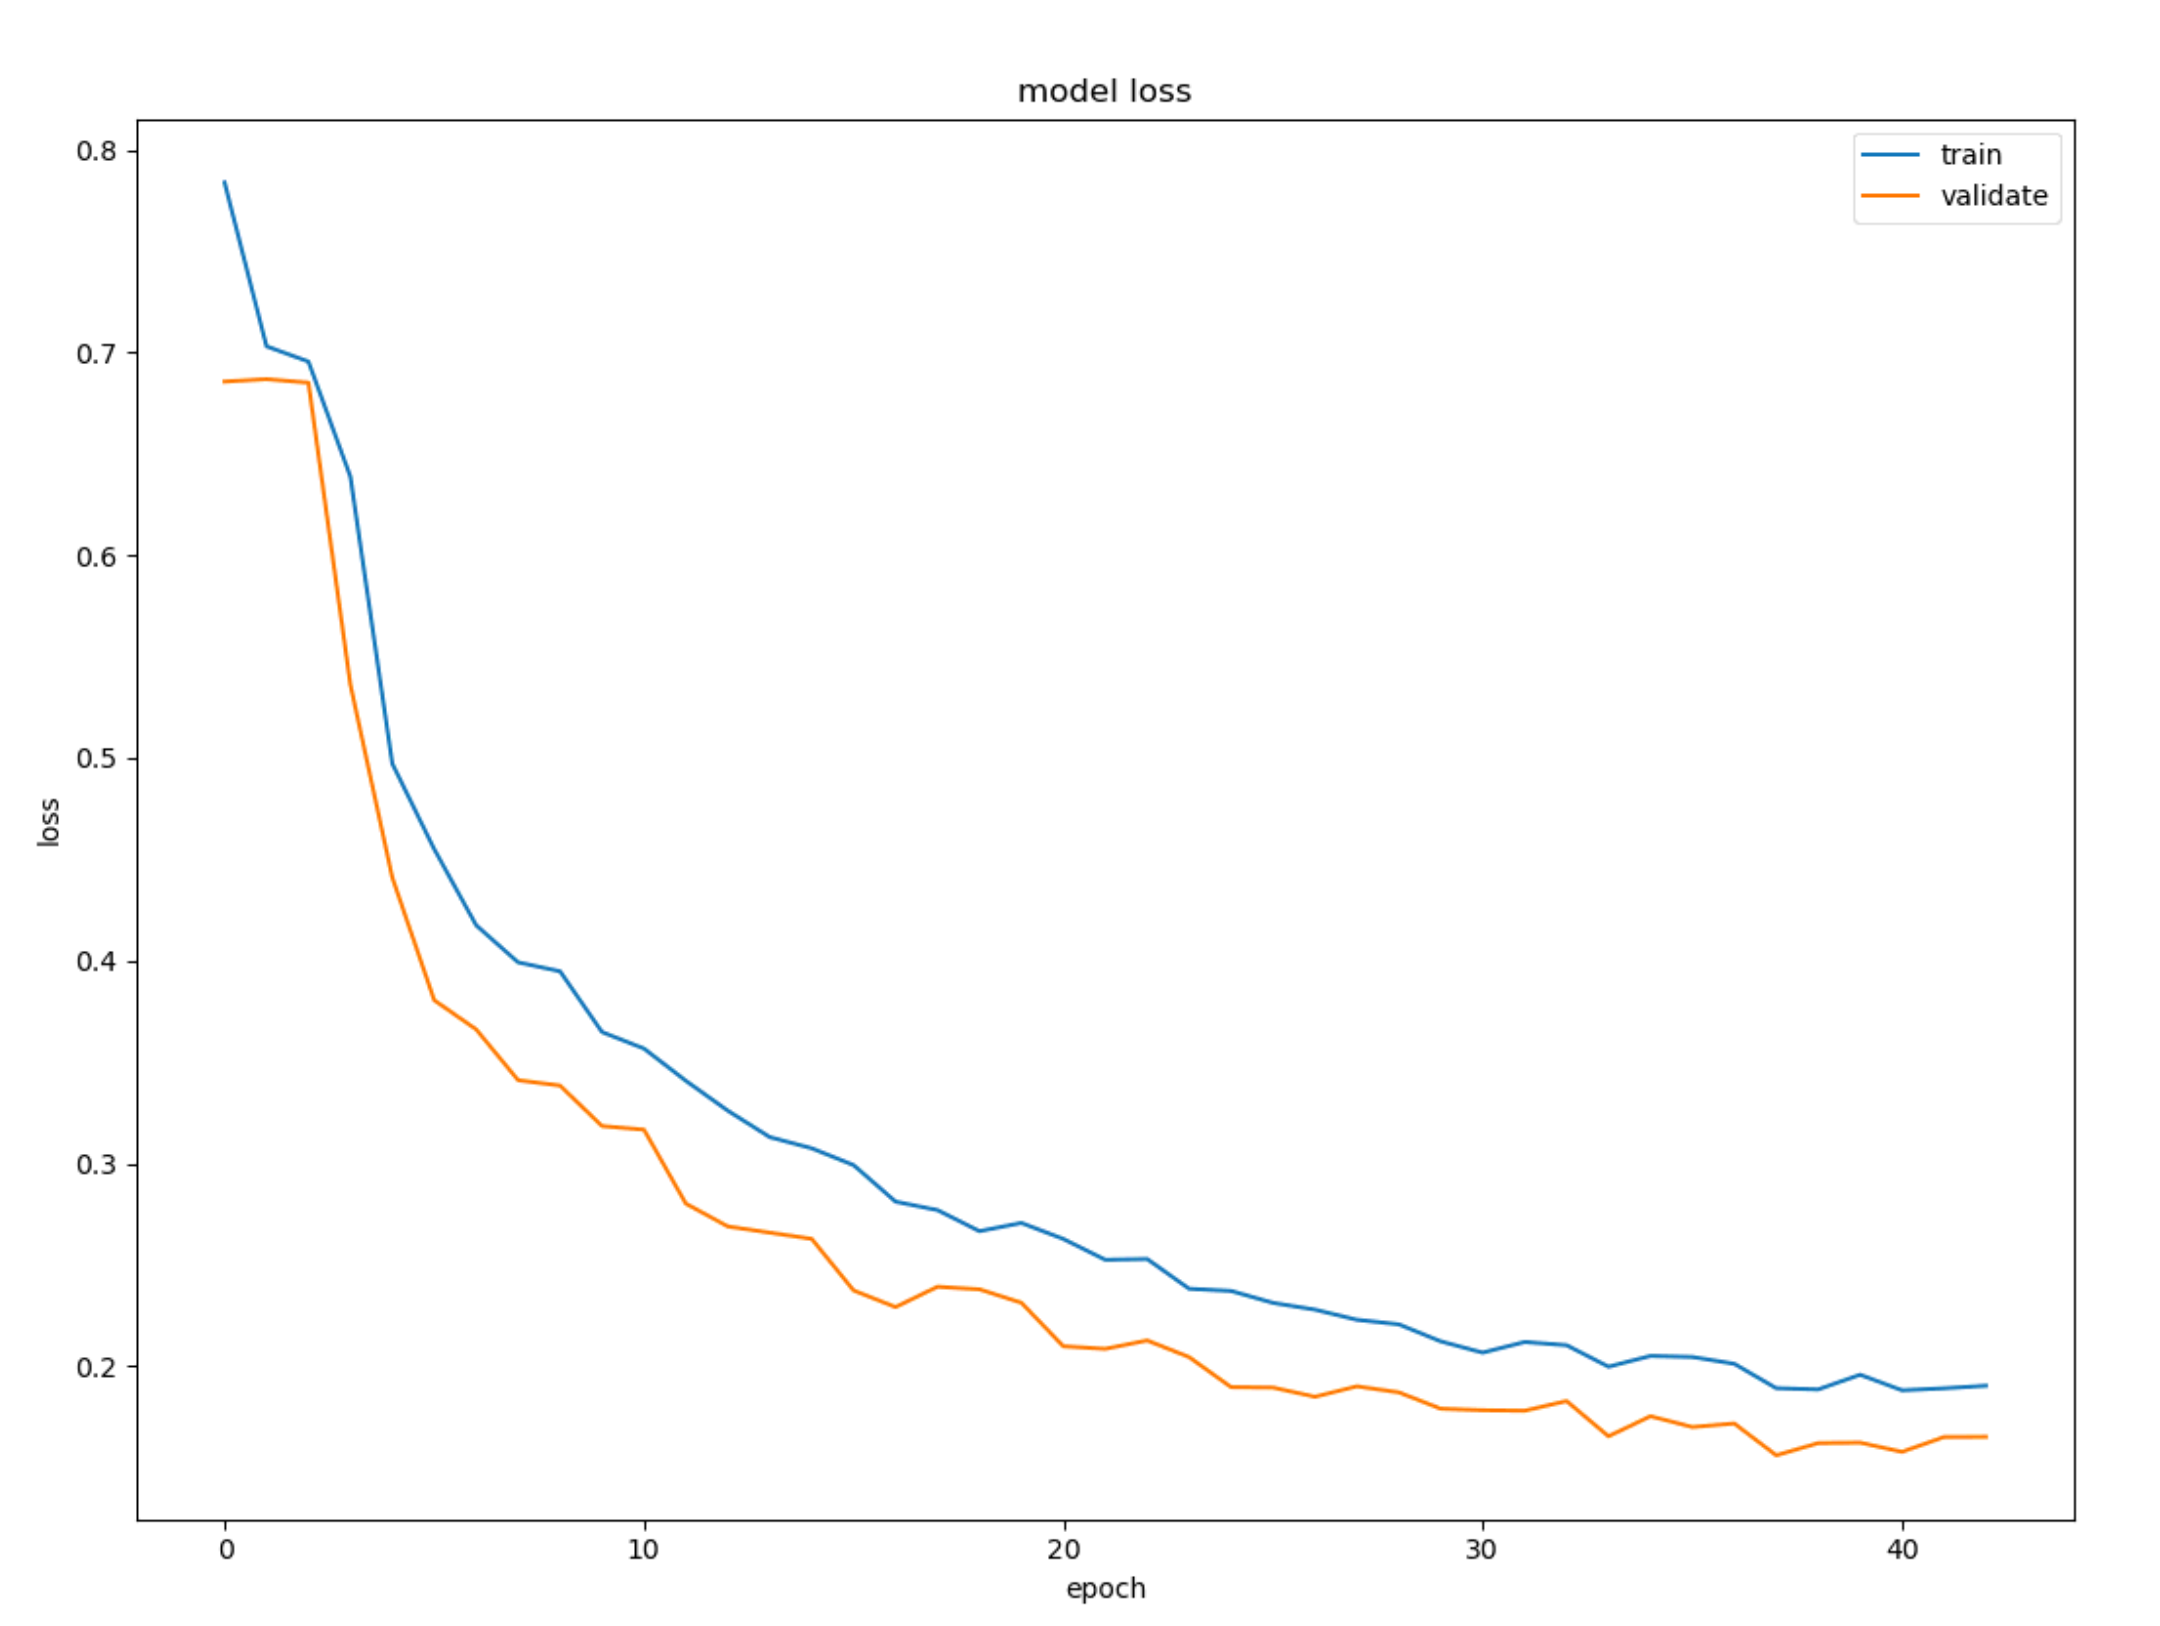
\includegraphics[width=8cm]{img/model_bench/latent.png}
\caption{Latent model loss}
\label{Latent model loss}
\end{minipage}
\end{figure}

\begin{figure}[!h]
\begin{minipage}{8cm}
\centering
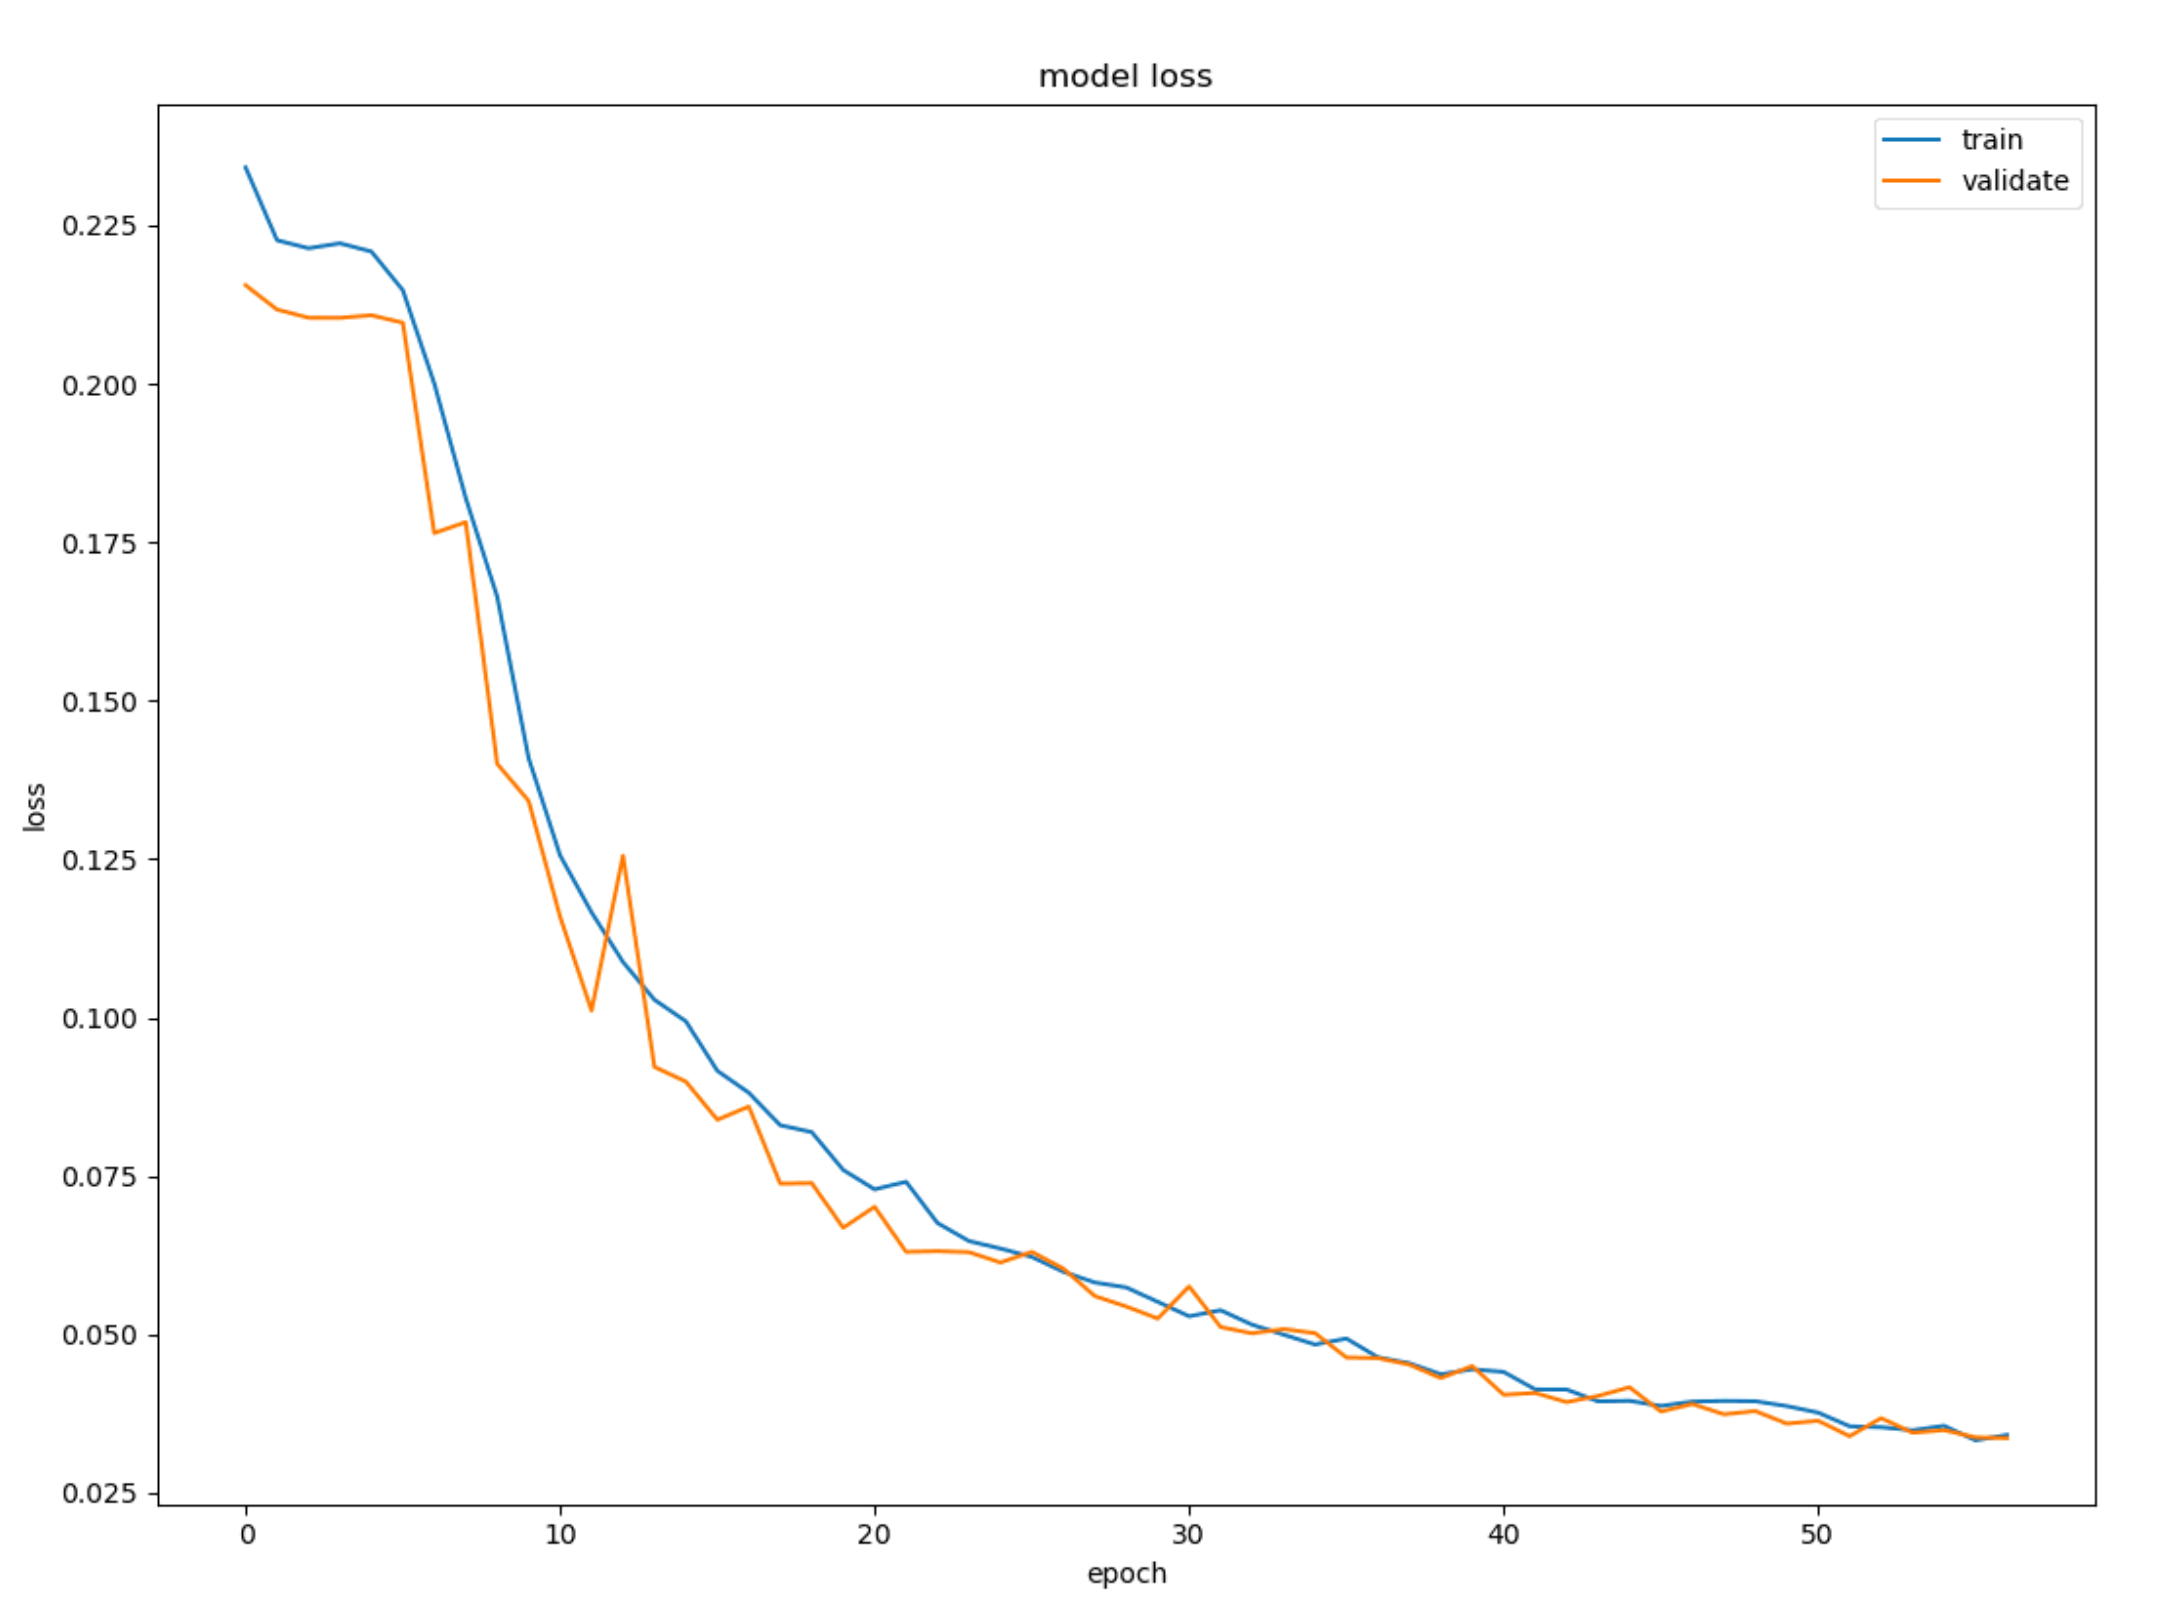
\includegraphics[width=8cm]{img/model_bench/rnn.png}
\caption{RNN model loss}
\label{RNN model loss}
\end{minipage}
\hspace*{1cm}
\begin{minipage}{8cm}
\centering
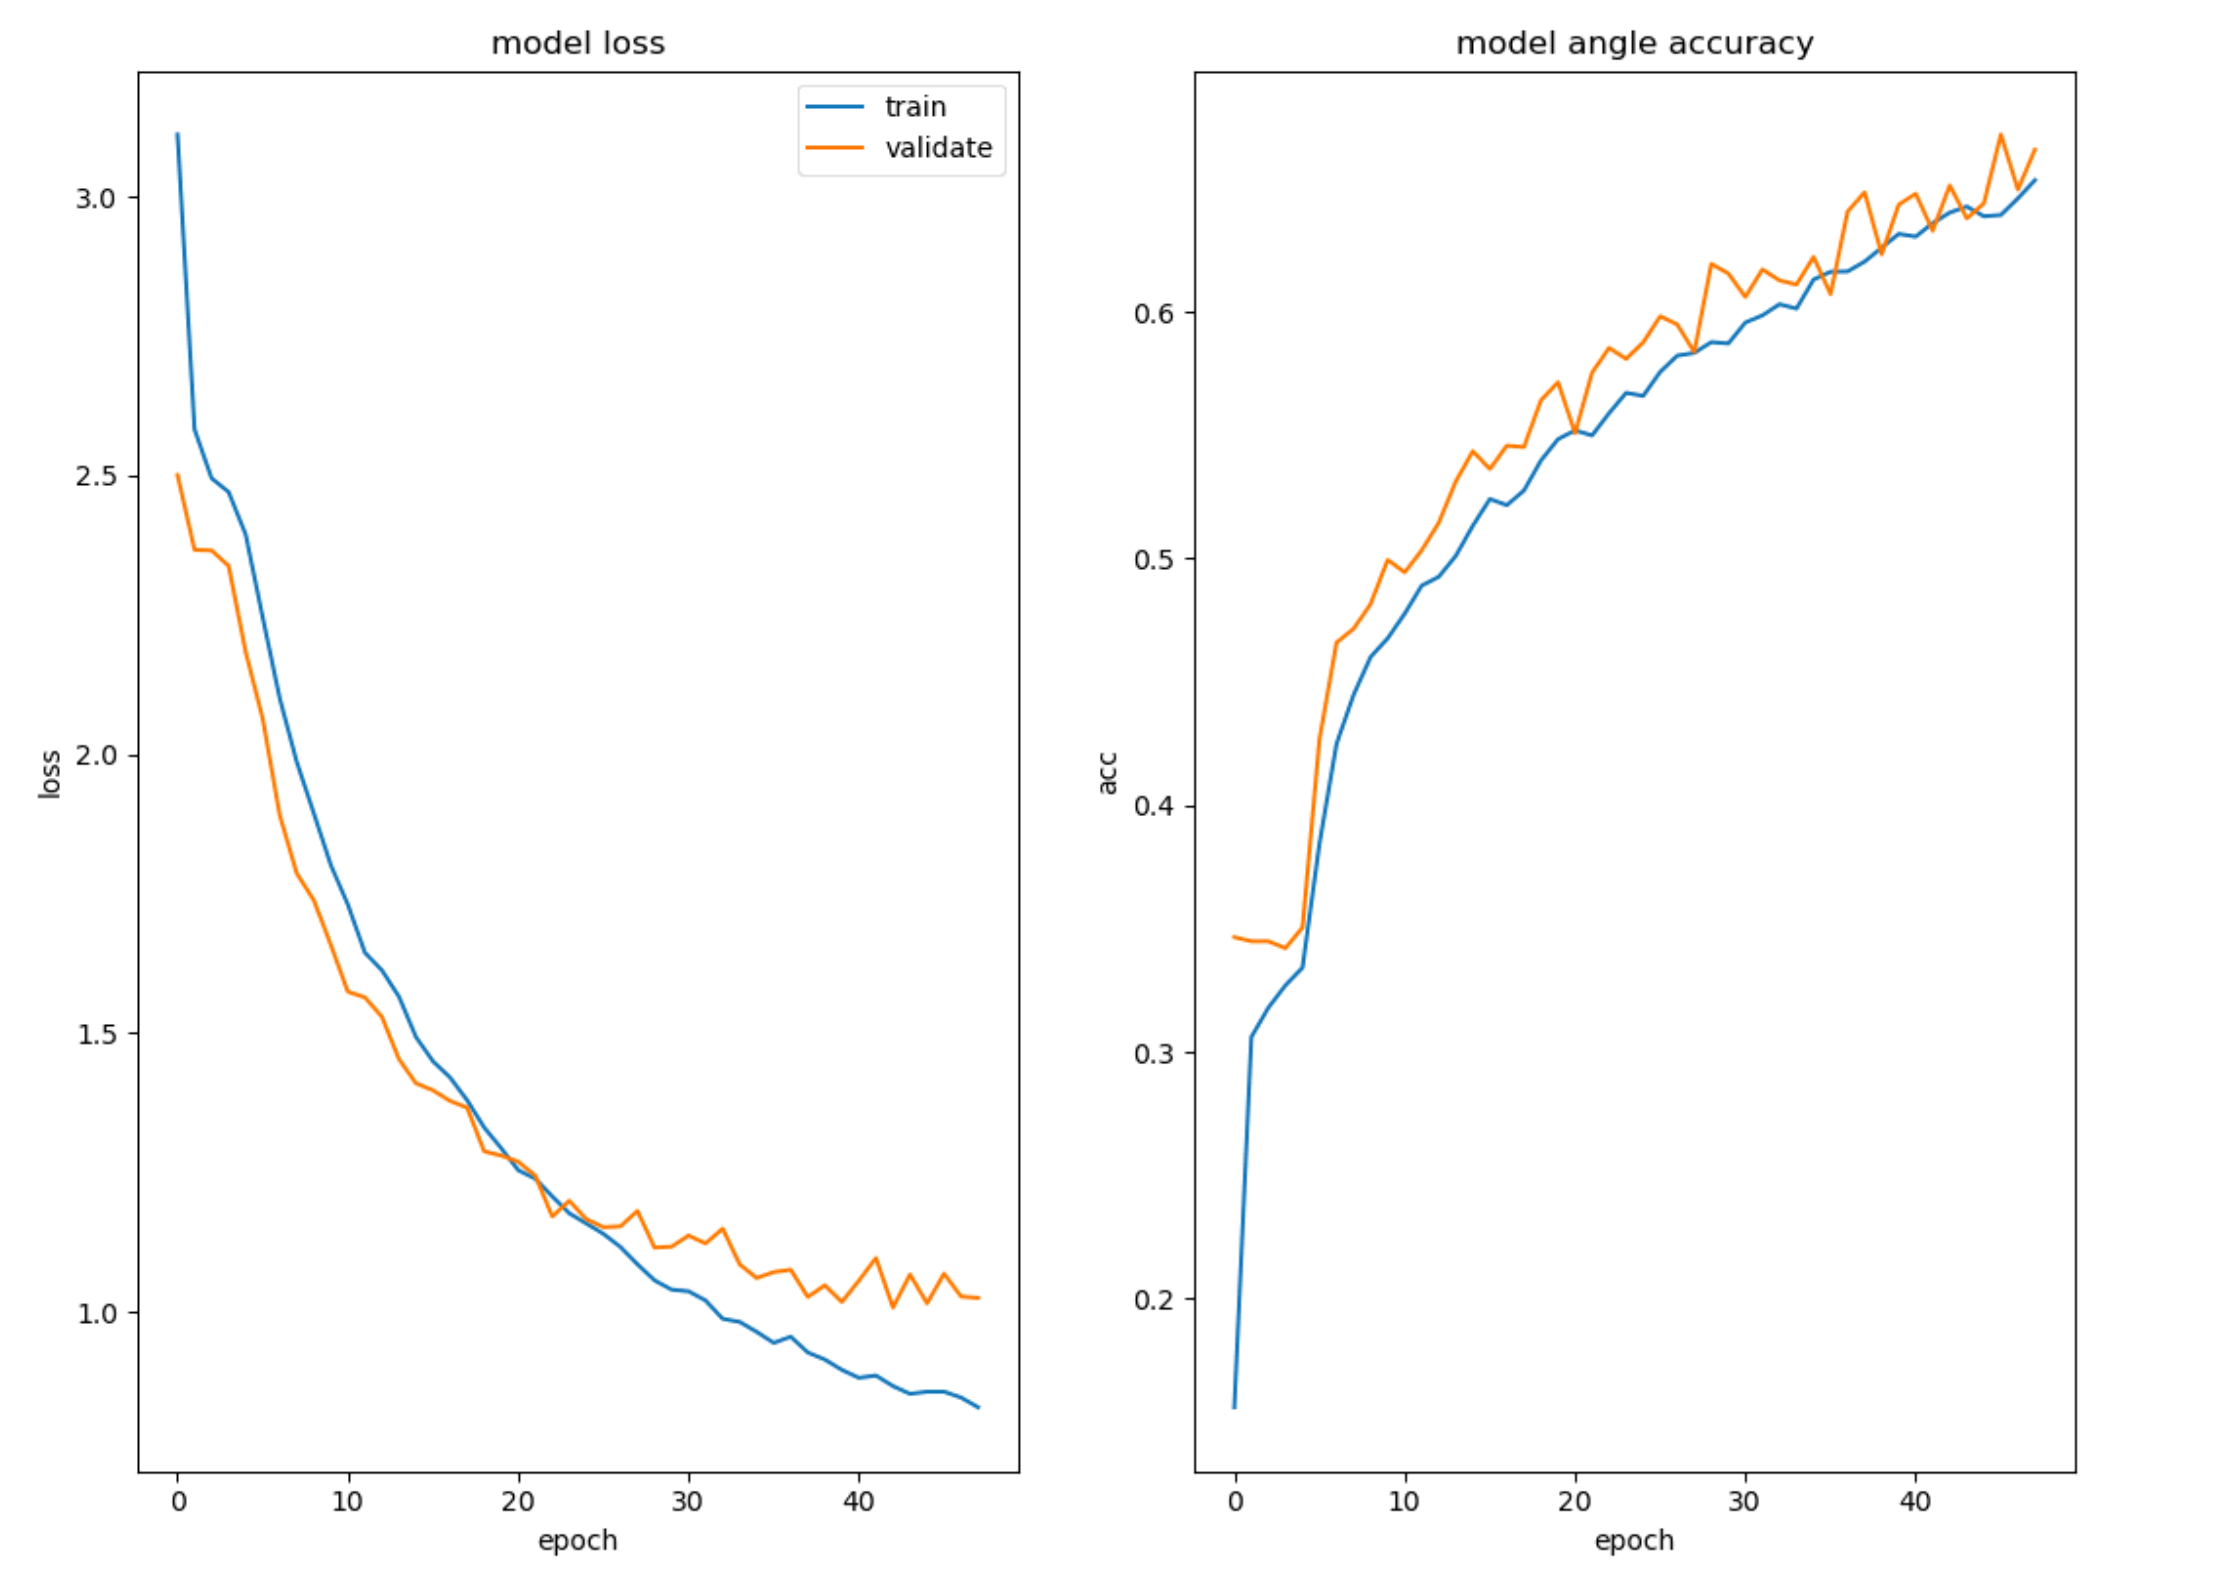
\includegraphics[width=8cm]{img/model_bench/categorical.png}
\caption{Categorical model loss and model angle loss}
\label{Categorical model loss}
\end{minipage}
\end{figure}

We can see that the \textbf{Linear} (Fig. \ref{Linear model loss}) and \textbf{RNN} (Fig.  \ref{RNN model loss}) model we used fit pretty well the data, but in the other hand, the \textbf{latent} (Fig. \ref{Latent model loss}) model tend to underfit the data while the \textbf{Categorical} (Fig. \ref{Categorical model loss}) model seems to overfit it.\footnote{The categorical model has 2 plot, one for the model angle accuracy and one for the model itself, that's because it's first trained on angle only and then on both throttle and angle.} \\

Even though the linear model look pretty well suited for the task, in practice, we found that it tends to oscilate way more than the RNN model. A solution to this kind of problem would be to implement a PID controler to smooth the driving, but this will be a way of improvement for the final model. 
\clearpage
\begin{figure}[H]
\centering
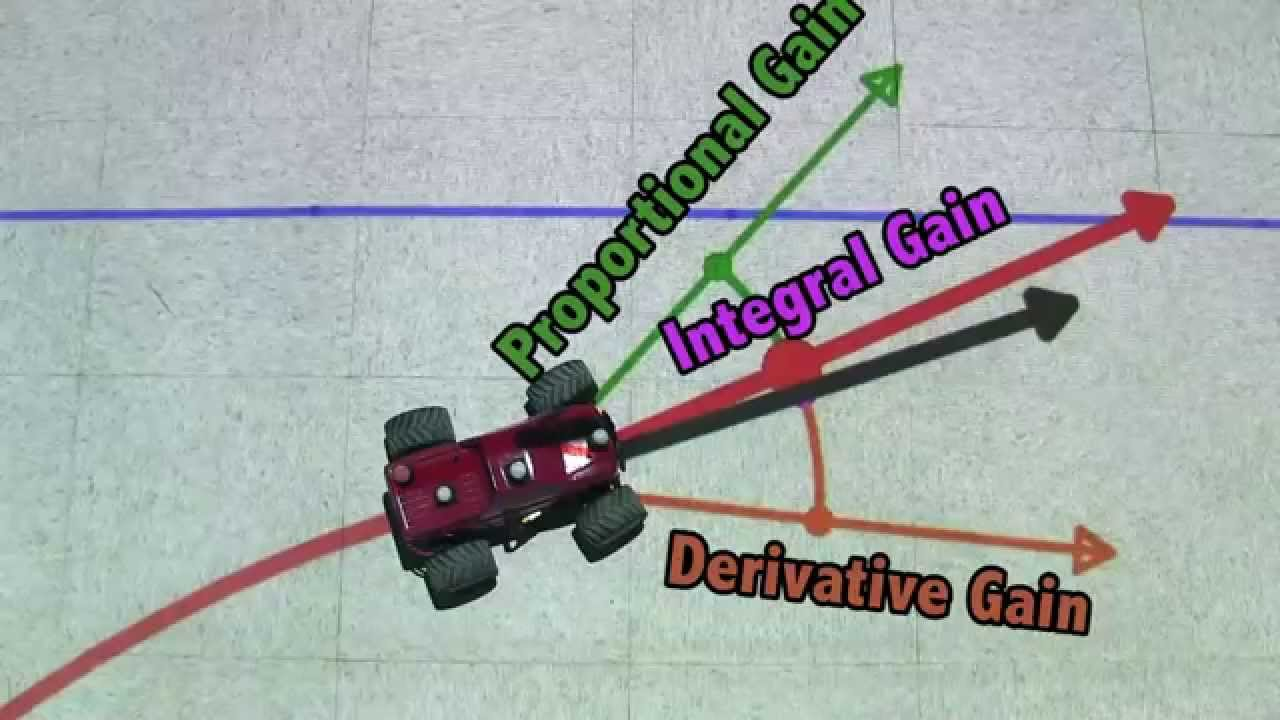
\includegraphics[scale=0.3]{img/PID.jpeg}
\caption{A PID Controler}
\end{figure}









\clearpage


\section{Conclusion}
This applicative project and first part of the sigma racing was very interesting. \\
We learned a lot and we now know that we are really pasionate about image recognition and deep learning.\\

It is a very complex domain and we are far from mastering it. Nevertheless, we have done our best in order to make a working model. We took deep learning online classes and read books to complete our train. It seemed, at first, very complexe (mostly the mathematicals aspects, and its still is !) but we managed to understand the basics and we are learning more every days.\\

This project will come to an end on June 2021. The next step is to buy the car and implement all the work that we have done inside it. We also plan to design our own removable track with the same specifications as the official one in order to test the car in different track configurations. Moreover, we will need to get cracking on the obstacles detections (is a Lidar sensor usefull ?) as well as the start and finish behaviors of the car.\\

We are still struggling with the hardware as we cannot borrow a GPU for the schools servers. It has a direct affect on the duration of the training and some help in this area would be more than welcome.

\hfill \\ 

\begin{figure}[!h]
\centering

\includegraphics[scale=0.15]{img/girou_barbault.jpg}
\caption{Romain (left) and Cyprien (right)}
\end{figure}
\clearpage
\clearpage
\section{List of Figure and Tables}
\listoffigures
\listoftables
\clearpage
\section{Bibliography}
\nocite{*}
\bibliographystyle{plain}
\bibliography{bib}
\begin{appendices}
\subsection{Code for the Lane Detection algorithm}\label{laneDetect}
\begin{python}
import cv2
import numpy as np
 
def make_points(image, line):
    slope, intercept = line
    y1 = int(image.shape[0])# bottom of the image
    y2 = int(y1*3/5)         # slightly lower than the middle
    x1 = int((y1 - intercept)/slope)
    x2 = int((y2 - intercept)/slope)
    return [[x1, y1, x2, y2]]
 
def average_slope_intercept(image, lines):
    left_fit    = []
    right_fit   = []
    if lines is None:
        return None
    for line in lines:
        for x1, y1, x2, y2 in line:
            fit = np.polyfit((x1,x2), (y1,y2), 1)
            slope = fit[0]
            intercept = fit[1]
            if slope < 0: # y is reversed in image
                left_fit.append((slope, intercept))
            else:
                right_fit.append((slope, intercept))
    # add more weight to longer lines

    if len(left_fit) and len(right_fit):
    #over-simplified if statement (should give you an idea of why the error occurs)
       left_fit_average  = np.average(left_fit, axis=0)
       right_fit_average = np.average(right_fit, axis=0)
       left_line  = make_points(image, left_fit_average)
       right_line = make_points(image, right_fit_average)
       averaged_lines = [left_line, right_line]
       return averaged_lines
 
def canny(img):
    gray = cv2.cvtColor(img, cv2.COLOR_RGB2GRAY)
    kernel = 5
    blur = cv2.GaussianBlur(gray,(kernel, kernel),0)
    canny = cv2.Canny(gray, 50, 150)
    return canny
 
def display_lines(img,lines):
    line_image = np.zeros_like(img)
    if lines is not None:
        for line in lines:
            for x1, y1, x2, y2 in line:
                cv2.line(line_image,(x1,y1),(x2,y2),(0,255,0),10)
    return line_image
 
def region_of_interest(canny):
    height = canny.shape[0]
    width = canny.shape[1]
    mask = np.zeros_like(canny)
 
    triangle = np.array([[
    (200, height),
    (550, 250),
    (1100, height),]], np.int32)
 
    cv2.fillPoly(mask, triangle, 255)
    masked_image = cv2.bitwise_and(canny, mask)
    return masked_image
 

# Code for the detection in an image named 'test_image.jpg'
image = cv2.imread('test_image.jpg')
lane_image = np.copy(image)
lane_canny = canny(lane_image)
cropped_canny = region_of_interest(lane_canny)
lines = cv2.HoughLinesP(cropped_canny, 2, np.pi/180, 100, np.array([]), minLineLength=40,maxLineGap=5)
averaged_lines = average_slope_intercept(image, lines)
line_image = display_lines(lane_image, averaged_lines)
combo_image = cv2.addWeighted(lane_image, 1, line_image, 1, 1)
cv2.imshow("result", combo_image)
cv2.waitKey(0)
cv2.destroyAllWindows()

# Code for the detection in a video named 'test2.mp4'
#cap = cv2.VideoCapture("test2.mp4")
#while(cap.isOpened()):
#    _, frame = cap.read()
#    canny_image = canny(frame)
#    cropped_canny = region_of_interest(canny_image)
#    lines = cv2.HoughLinesP(cropped_canny, 2, np.pi/180, 100, np.array([]), minLineLength=40,maxLineGap=5)
#    averaged_lines = average_slope_intercept(frame, lines)
#    line_image = display_lines(frame, averaged_lines)
#    combo_image = cv2.addWeighted(frame, 0.8, line_image, 1, 1)
#    cv2.imshow("result", combo_image)
#    if cv2.waitKey(1) & 0xFF == ord('q'):
#        break
#cap.release()
#cv2.destroyAllWindows()
\end{python}
\clearpage

\subsection{Image at each step in the lane detect algorithm}
\label{imagelaneDetect}
\begin{figure}[!h]
\begin{minipage}{7cm}
\centering
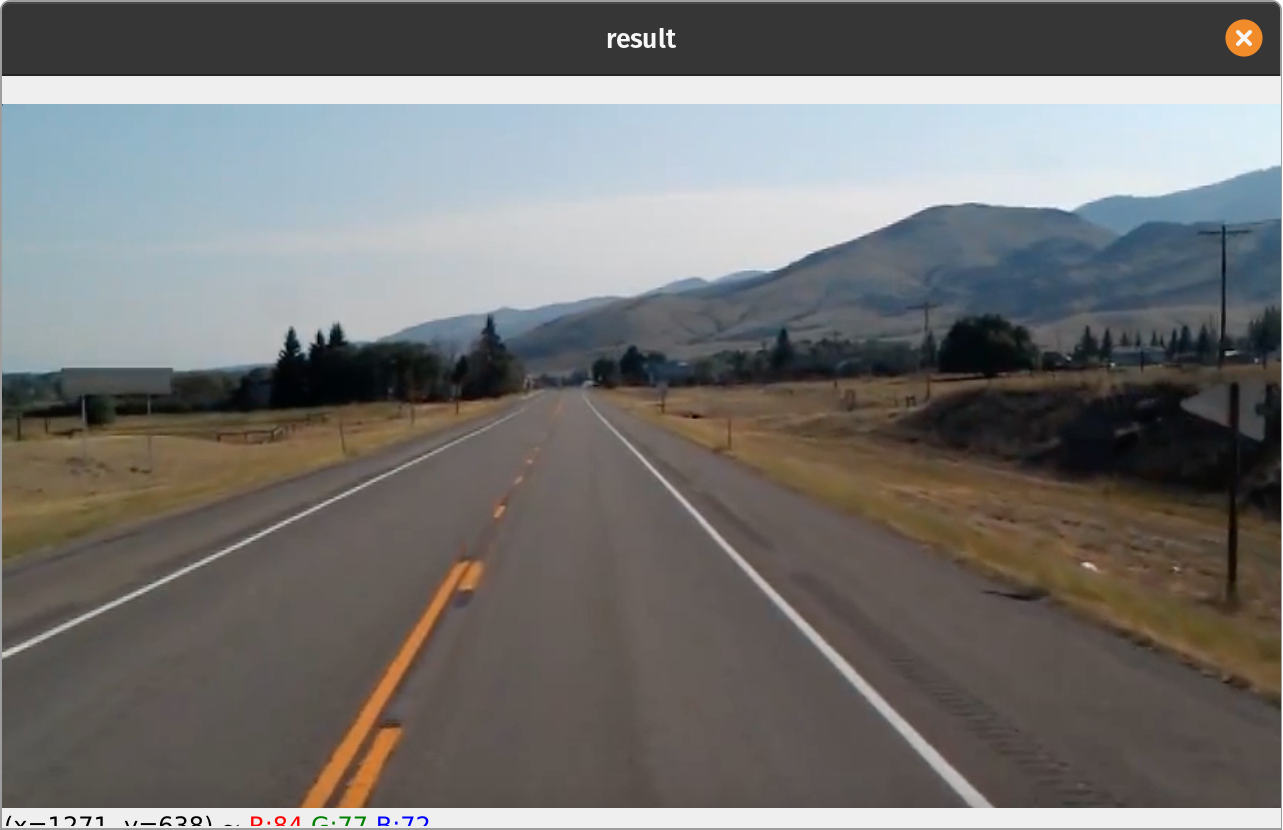
\includegraphics[width=6cm]{img/lane_detect/lane_img.png}
\caption{Original Image}
\end{minipage}
\hspace*{1cm}
\begin{minipage}{7cm}
\centering
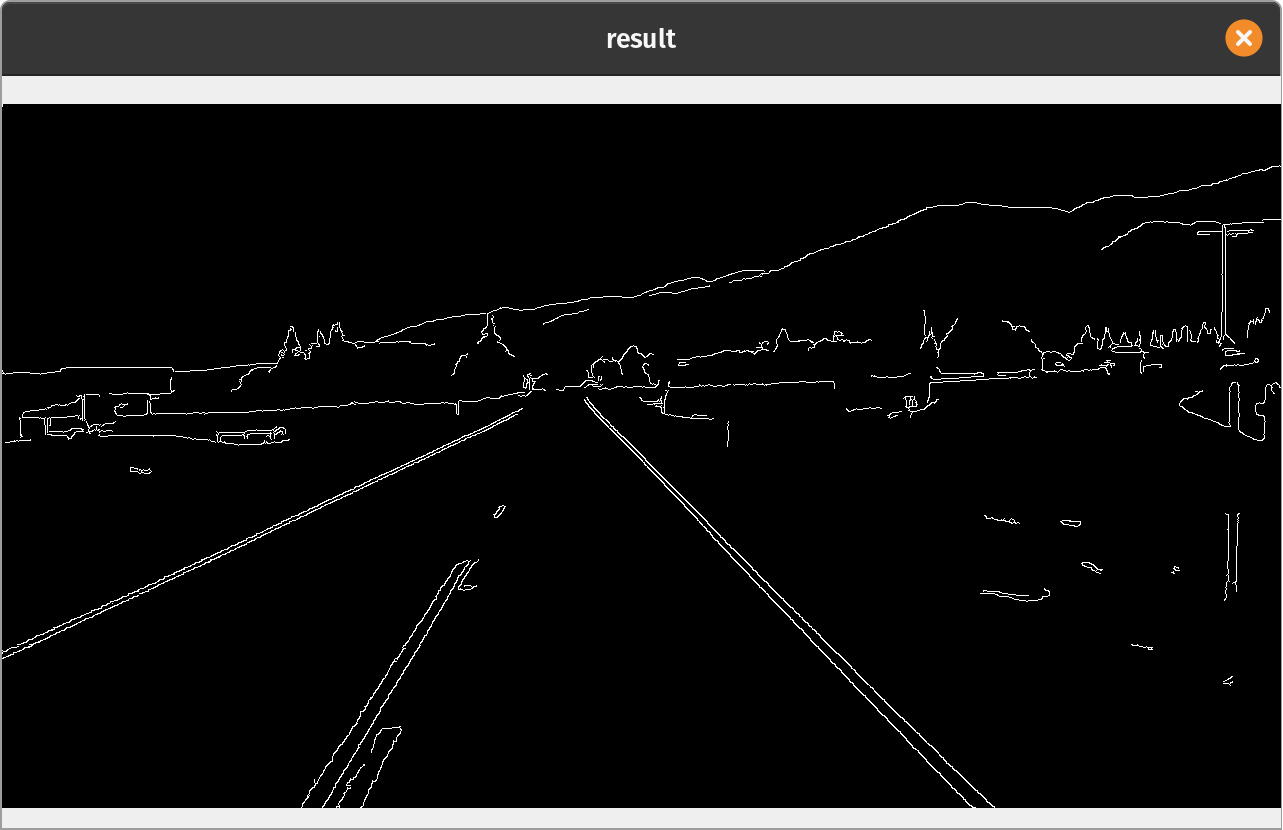
\includegraphics[width=6cm]{img/lane_detect/canny_img.png}
\caption{Gray Image after applying blur and canny-edge detection}
\end{minipage}
\end{figure}

\begin{figure}[!h]
\begin{minipage}{7cm}
\centering
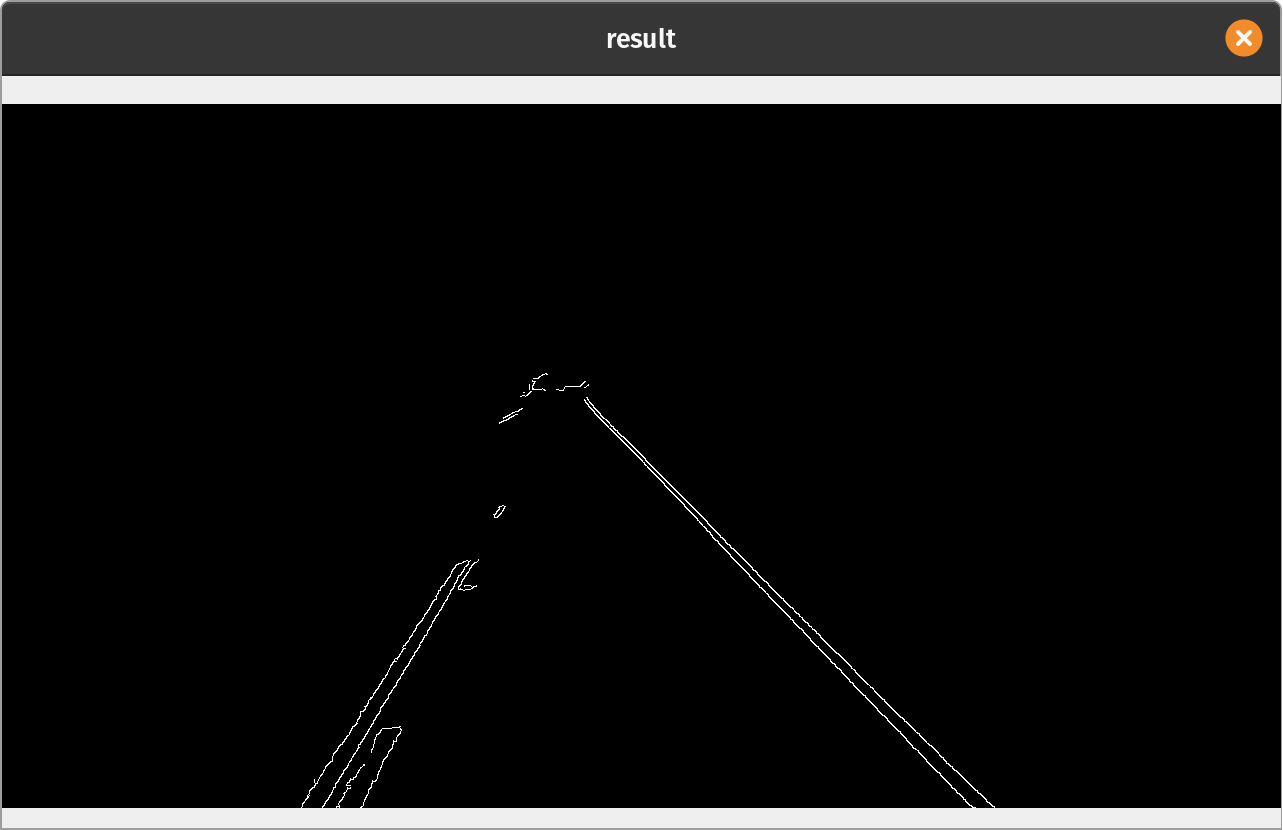
\includegraphics[width=6cm]{img/lane_detect/cropped_img.png}
\caption{We cropped the image to the center triangle}
\end{minipage}
\hspace*{1cm}
\begin{minipage}{7cm}
\centering
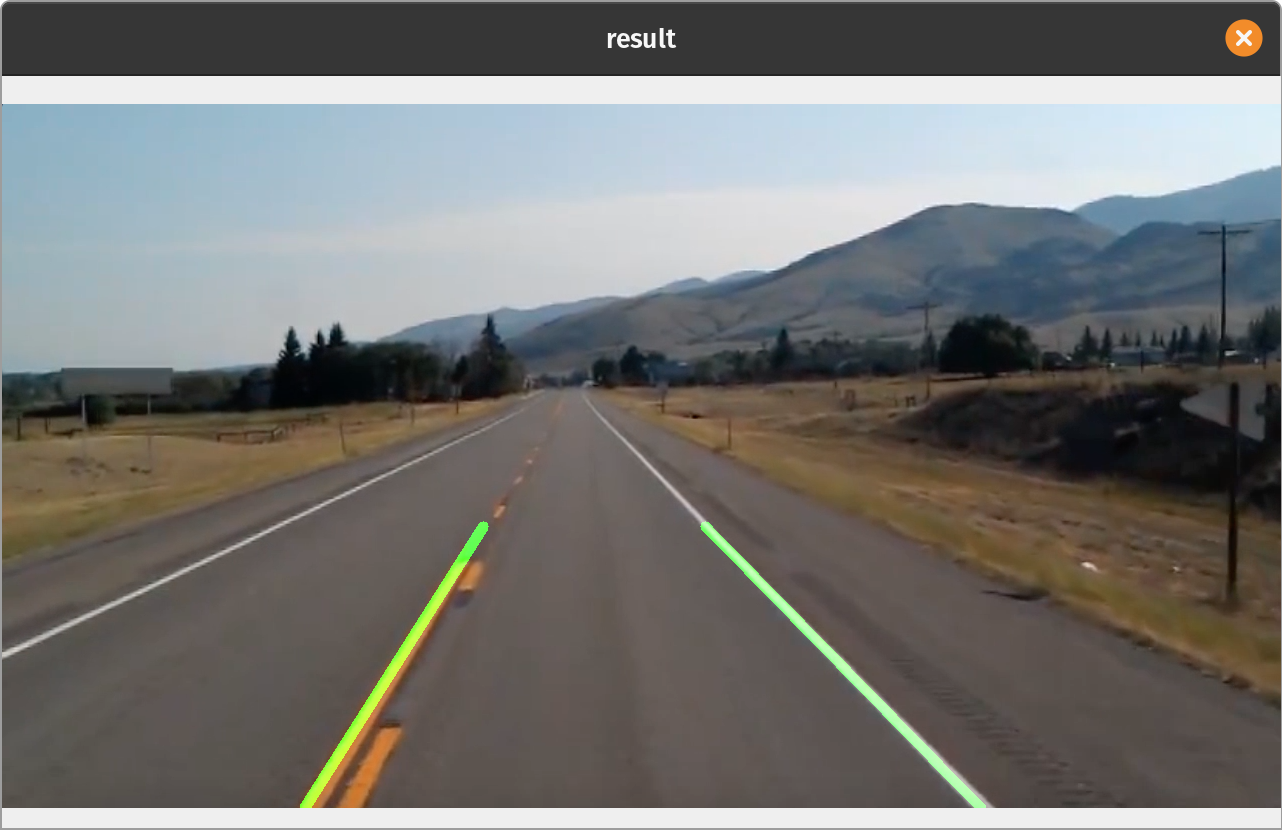
\includegraphics[width=6cm]{img/lane_detect/combo_img.png}
\caption{Final image with superposed detected lines (in green)}
\end{minipage}
\end{figure}

\clearpage
\subsection{TCP Client in Python}
\label{TCPClient}
\begin{python}
import socket
import base64
import requests
import socketio
import sys
import time
import json


# specify Host and Port
HOST = 'localhost'
PORT = 9091


def send_data(steering, throttle, brake):
    msg = str('{"msg_type": "control", "steering": "' +
              str(steering) + '","throttle": "' + str(throttle) +
              '","brake": "' + str(brake) + '"}').encode('utf-8')
    soc.sendall(msg)


def recv_full():
    """
    Test if the msg_type is telemetry, if yes, return the data
    """
    for _ in range(2):
        data = json.loads(soc.recv(8192).decode('utf-8'))
        if not data:
            break
        if data['msg_type'] == 'car_loaded':
            continue
        return json.loads(soc.recv(5000).decode('utf-8'))


def write_data():
    data = recv_full()
    with open('image.jpg', 'wb') as image:
        image.write(base64.b64decode(data['image']))
    with open("data.json", 'w') as f:
        json.dump(data, f)



with socket.socket(socket.AF_INET, socket.SOCK_STREAM) as soc:
    soc.connect((HOST, PORT))
    write_data()



sio = socketio.Client()
\end{python}

\subsection{Financial Management Report}
Next, you can find the financial management report we had to do, inside you will find an overview of the project and the differents approach we took for the budget repartition and the choice of the components of the car.
\includepdf[pages=-]{pdf/PA_finance.pdf}

\end{appendices}
\end{document}
